%%% Use option "handout" to disable pause/action
\documentclass{beamer}
%\documentclass[handout]{beamer}
\usepackage[utf8]{inputenc}
\usepackage{utopia}
\usetheme{Madrid}
\usecolortheme{default}

% packages
\usepackage{colortbl}
\usepackage{etoolbox}
\usepackage[square,numbers,sort&compress]{natbib}
\usepackage{algorithm}
\usepackage{algorithmic}
\usepackage{booktabs}
\usepackage{rotating}
\usepackage{adjustbox}
\usepackage{xspace}
\usepackage{tcolorbox}
\usepackage{subfig}
\usepackage{hyperref}
\usepackage[capitalise,nosort,nameinlink]{cleveref}
\usepackage{tikz}
\usepackage{tikz-qtree}
\usepackage{circuitikz}
\usepackage{pgfplotstable}
\usetikzlibrary{positioning,arrows}
% Plots with BenchExec
\usepackage{standalone}
\usepackage[
      group-digits=integer, group-minimum-digits=4, % group digits by thousands
      free-standing-units, unit-optional-argument, % easier input of numbers with units
]{siunitx}
\usepackage{pgfplots}
\pgfplotsset{
      compat=1.9,
      %log ticks with fixed point, % no scientific notation in plots
      table/col sep=tab, % only tabs are column separators
      unbounded coords=jump, % better have skips in a plot than appear to be interpolating
      filter discard warning=false, % Don't complain about empty cells
}
\SendSettingsToPgf % use siunitx formatting settings in PGF, too
% end packages

% symbols
\newcommand{\booldom}{\mathbb{B}} % Boolean domain
\newcommand{\limply}{\rightarrow} % logical implication
\newcommand{\vl}[1]{\texttt{var}(#1)} % variable of a literal
\newcommand{\as}{\tau} % an assignment
\newcommand{\av}[1]{\mathcal{A}(#1)} % all assignments over a variable set
\newcommand{\pf}{\phi} % propositional formula (quantifier-free)
\newcommand{\vf}[1]{\texttt{vars}(#1)} % variable of a formula
\newcommand{\pcf}[2]{#1|_{#2}} % positive cofactor
\newcommand{\ncf}[2]{#1|_{\lnot#2}} % negative cofactor
\newcommand{\Qf}{\Phi} % quantified formula
\newcommand{\base}{X_d} % a base set of a formula
\newcommand{\random}[1]{\rotatebox[origin=c]{180}{$\mathsf{R}$}^{#1}} % randomized quantifier
\newcommand{\spb}[1]{\Pr[#1]} % satisfying probability
\newcommand{\wt}{\omega} % weight of a variable
\newcommand{\sat}[1]{\texttt{SAT}(#1)} % formula is satisfiable
\newcommand{\unsat}[1]{\texttt{UNSAT}(#1)} % formula is unsatisfiable
\newcommand{\model}[1]{#1.\mathrm{model}} % formula is unsatisfiable
\newcommand{\select}{\psi} % selection formula
\newcommand{\cx}{C^X} % sub-clause of X variables
\newcommand{\cy}{C^Y} % sub-clause of Y variables
\newcommand{\sv}[1]{s_{#1}} % selection variable
\newcommand{\dep}[1]{D_{#1}} % dependency set
\newcommand{\uvs}{V_{\Qf}^{\forall}} % universal variable set
\newcommand{\evs}{V_{\Qf}^{\exists}} % existential variable set
\newcommand{\rvs}{V_{\Qf}^{\random{}}} % random variable set
\newcommand{\skf}{\mathcal{F}} % Skolem function set
\newcommand{\nodeval}[1]{#1.\mathrm{value}} % BDD node value
\newcommand{\nodevar}[1]{#1.\mathrm{var}} % BDD node variable
\newcommand{\nodevisit}[1]{#1.\mathrm{visited}} % BDD node visited flag
\newcommand{\nodethen}[1]{#1.\mathrm{then}} % BDD node then
\newcommand{\nodeelse}[1]{#1.\mathrm{else}} % BDD node else
\newcommand{\nodesp}[1]{#1.\mathrm{sp}} % BDD node satisfying probability
\newcommand{\er}{\epsilon} % error rate of a gate
\newcommand{\dr}{\delta} % defect rate of a design
\DeclareMathOperator*{\argmax}{arg\,max} % maximizing argument
\DeclareMathOperator*{\argmin}{arg\,min} % minimizing argument

% tools
\newcommand{\tool}[1]{\texttt{#1}\xspace}
\newcommand{\definetool}[2]{\newcommand{#1}{\tool{#2}}\xspace}
\definetool{\ressat}{reSSAT}
\definetool{\ressatb}{reSSAT-b}
\definetool{\erssat}{erSSAT}
\definetool{\erssatb}{erSSAT-b}
\definetool{\bddsp}{BDDsp}
\definetool{\bddspnr}{BDDsp-nr}
\definetool{\maxplan}{MAXPLAN}
\definetool{\zander}{ZANDER}
\definetool{\dcssat}{DC-SSAT}
\definetool{\complan}{ComPlan}
\definetool{\minisat}{MiniSat}
\definetool{\cachet}{Cachet}
\definetool{\approxmc}{ApproxMC}
\definetool{\ctwod}{c2d}
\definetool{\dpmc}{DPMC}
\definetool{\procount}{ProCount}
\definetool{\cnfgen}{CNFgen}
\definetool{\benchexec}{BenchExec}
\definetool{\abc}{ABC}
\definetool{\cudd}{CUDD}
\definetool{\prism}{PRISM}
\definetool{\timeout}{TO}
\definetool{\memout}{MO}

% URL
\newcommand{\ssatabcurl}{https://github.com/NTU-ALComLab/ssatABC}
\newcommand{\ssatbenchmarkurl}{https://github.com/NTU-ALComLab/ssat-benchmarks}
\newcommand{\benchexecurl}{https://github.com/sosy-lab/benchexec}

% Evaluation setup, environment, and version
\newcommand{\machineSpec}{one 2.2\,GHz CPU (Intel Xeon Silver 4210) with 40~processing units and \num{134616}\,MB of RAM}
\newcommand{\osInfo}{Ubuntu~20.04 (64~bit), running Linux~5.4}
\newcommand{\compiler}{\texttt{g++ 9.3.0}}
\newcommand{\timelimit}{\SI{15}{min}}
\newcommand{\memlimit}{\SI{15}{GB}}
\newcommand{\ssatABCRevision}{commit \texttt{2ff8e74} of branch \texttt{master}\xspace}
\newcommand{\ssatBenchRevision}{commit \texttt{ea9fbae} of branch \texttt{master}\xspace}

% constant words
\newcommand{\word}[1]{\textsc{#1}\xspace}
\newcommand{\defineword}[2]{\newcommand{#1}{\word{#2}}\xspace}
\defineword{\true}{true}
\defineword{\false}{false}
\defineword{\disjoin}{or}
\defineword{\conjoin}{and}
\defineword{\nand}{nand}
\defineword{\xor}{xor}

% customize package "amsthm"
\renewcommand\qedsymbol{$\blacksquare$}

% customize package "cleveref"
\newcommand{\creflastconjunction}{, and~}
\crefname{equation}{Eq.}{Eqs.}
\crefname{algorithm}{Alg.}{Algs.}
\crefname{line}{line}{lines}
\crefalias{ALC@unique}{line}
\crefalias{ALC@line}{line}

% customize package "algorithmic"
\renewcommand{\algorithmicrequire}{\textbf{Input:}}
\renewcommand{\algorithmicensure}{\textbf{Output:}}

% customize package "pgfplotstable"
\pgfplotstableset{
      circuit column/.style={
                  /pgfplots/table/display columns/#1/.style={
                              string type,column type=l,column name=\textsc{Circuit}
                        }
            },
      formula column/.style={
                  /pgfplots/table/display columns/#1/.style={
                              string type,column type=l,column name=\textsc{Formula}
                        }
            },
      pi column/.style={
                  /pgfplots/table/display columns/#1/.style={fixed,column type=r,column name=\#PI}
            },
      ai column/.style={
                  /pgfplots/table/display columns/#1/.style={fixed,column type=r,column name=\#AI}
            },
      po column/.style={
                  /pgfplots/table/display columns/#1/.style={fixed,column type=r,column name=\#PO}
            },
      and column/.style={
                  /pgfplots/table/display columns/#1/.style={fixed,column type=r,column name=\#And}
            },
      level column/.style={
                  /pgfplots/table/display columns/#1/.style={fixed,column type=r,column name=\#Level}
            },
      time column/.style={
                  /pgfplots/table/display columns/#1/.style={
                              string replace={nan}{},sci,sci zerofill,sci sep align,precision=2,sci e,column name=T (s)
                        }
            },
      prob column/.style={
                  /pgfplots/table/display columns/#1/.style={
                              string replace={nan}{},sci,sci zerofill,sci sep align,precision=2,sci e,column name=$\Pr$
                        }
            },
      ubound column/.style={
                  /pgfplots/table/display columns/#1/.style={
                              string replace={nan}{},sci,sci zerofill,sci sep align,precision=2,sci e,column name=UB
                        }
            },
      lbound column/.style={
                  /pgfplots/table/display columns/#1/.style={
                              string replace={nan}{},sci,sci zerofill,sci sep align,precision=2,sci e,column name=LB
                        }
            },
      ubtime column/.style={
                  /pgfplots/table/display columns/#1/.style={
                              string replace={nan}{},sci,sci zerofill,sci sep align,precision=2,sci e,column name=T-UB (s)
                        }
            },
      lbtime column/.style={
                  /pgfplots/table/display columns/#1/.style={
                              string replace={nan}{},sci,sci zerofill,sci sep align,precision=2,sci e,column name=T-LB (s)
                        }
            }
}

% Fix line counters if multiple algorithms exist
\makeatletter % Make '@' a normal letter so that it can be used in *.tex files
\@addtoreset{ALC@line}{algorithm}
\@addtoreset{ALC@unique}{algorithm}
\makeatother % Undo the change to '@'

% Title page information
\title[Stochastic Boolean Satisfiability]{Stochastic Boolean Satisfiability}
\subtitle{Decision Procedures, Generalization, and Applications}

\author[Nian-Ze Lee]{Nian-Ze Lee\\~\\{\footnotesize Advisor: Prof. Jie-Hong Roland Jiang}}

\institute[NTU GIEE]{Graduate Institute of Electronics Engineering, National Taiwan University}

\date[Oral Defense, Jun. 2021]{Doctoral Dissertation Oral Defense, 2nd June 2021}

\setbeamerfont{section in toc}{size=\footnotesize}
\setbeamerfont{subsection in toc}{size=\scriptsize}

\makeatletter
\patchcmd{\beamer@sectionintoc}{\vskip1.5em}{\vskip0.5em}{}{}
\makeatother

\AtBeginSection[]
{
      \begin{frame}
            \frametitle{Outline}
            \tableofcontents[currentsection,hideallsubsections]
      \end{frame}
}

\AtBeginSubsection[]
{
      \begin{frame}
            \frametitle{Outline}
            \tableofcontents[currentsection,currentsubsection,subsectionstyle=show/shaded/hide]
      \end{frame}
}

\begin{document}

%---------------------------------------------------

\frontmatter
\begin{abstracten}{Stochastic Satisfiability, Probabilistic Design}
  \textit{Stochastic Boolean satisfiability} (SSAT) is an expressive language to formulate computational problems with randomness,
such as the inference of Bayesian networks,
propositional probabilistic planning,
and partially observable Markov decision process (POMDP).
Solving an SSAT formula lies in the PSPACE-complete complexity class,
the same as solving a \textit{quantified Boolean formula} (QBF).
Despite its broad applications and profound theoretical values,
SSAT has drawn relatively less attention compared to SAT or QBF.

We identify relevant applications of random-exist and exist-random SSAT solving to the formal verification of \textit{probabilistic design}.
Probabilistic design is an emerging computational paradigm to accept device variability in the nanometer regime of VLSI circuit fabrication.
We formulate the property evaluation of probabilistic design under the average-case and worst-case analyses with SSAT.

Motivated by the emerging applications of SSAT,
we propose novel algorithms to solve random-exist and exist-random quantified SSAT formulas.
These two fragments of SSAT have important AI applications in the reasoning of Bayesian networks and the search of an optimal strategy for probabilistic conformant planning.
In contrast to the conventional SSAT-solving approaches based on Davis-Putnam-Logemann-Loveland (DPLL) search,
we exploit modern techniques for SAT/QBF solving and model counting to improve the computational efficiency.
Moreover, unlike the prior DPLL-based exact algorithms for SSAT solving,
the proposed algorithms are able to solve an SSAT formula approximately by deriving bounds of its satisfying probability.

The proposed algorithms are implemented in the open-source SSAT solvers \ressat and \erssat.
Our evaluation shows that \ressat and \erssat solvers outperform the state-of-the-art SSAT solver on various formulas in both runtime and memory usage.
They also provide useful bounds for cases where the state-of-the-art solver fails to compute exact answers.

In spite of its various applications,
SSAT is limited by its descriptive power within the PSPACE complexity class.
More complex problems, such as the NEXPTIME-complete decentralized POMDP (Dec-POMDP), cannot be succinctly encoded with SSAT.
To provide a logical formalism for such problems,
we extend the \textit{dependency quantified Boolean formula} (DQBF),
a representative problem in the NEXPTIME-complete class,
to its stochastic variant, named \textit{dependency SSAT} (DSSAT),
and show that DSSAT is also NEXPTIME-complete.
We demonstrate the potential applications of DSSAT to the synthesis of probabilistic and approximate design and the encoding of Dec-POMDP problems.

%%% Abstract of the IJCAI '17 paper
\iffalse
    Stochastic Boolean Satisfiability (SSAT) is a powerful formalism to represent computational problems with uncertainty, such as belief network inference and propositional probabilistic planning. Solving SSAT formulas lies in the PSPACE-complete complexity class same as solving Quantified Boolean Formulas (QBFs). While many endeavors have been made to enhance QBF solving in recent years, SSAT has drawn relatively less attention. This paper focuses on random-exist quantified SSAT formulas, and proposes an algorithm combining modern satisfiability (SAT) techniques and model counting to improve computational efficiency. Unlike prior exact SSAT algorithms, the proposed method can be easily modified to solve approximate SSAT by deriving upper and lower bounds of satisfying probability. Experimental results show that our method outperforms the state-of-the-art algorithm on random $k$-CNF and AI-related formulas in both runtime and memory usage, and has effective application to approximate SSAT on VLSI circuit benchmarks.
\fi
%%% Abstract of the IJCAI '18 paper
\iffalse
    Stochastic Boolean satisfiability (SSAT) is an expressive language to formulate decision problems with randomness. Solving SSAT formulas has the same PSPACE-complete computational complexity as solving quantified Boolean formulas (QBFs). Despite its broad applications and profound theoretical values, SSAT has received relatively little attention compared to QBF. In this paper, we focus on exist-random quantified SSAT formulas, also known as E-MAJSAT, which is a special fragment of SSAT commonly applied in probabilistic conformant planning, posteriori hypothesis, and maximum expected utility. Based on clause selection, a recently proposed QBF technique, we propose an algorithm to solve E-MAJSAT. %Several enhancement techniques are also devised to improve the computational efficiency.
    Moreover, our method can provide an approximate solution to E-MAJSAT with a lower bound when an exact answer is too expensive to compute.
    Experiments show that the proposed algorithm achieves significant performance gains and memory savings over the state-of-the-art SSAT solvers on a number of benchmark formulas, and provides useful lower bounds for cases where prior methods fail to compute exact answers.
\fi
%%% Abstract of the TC '18 paper
\iffalse
    In the nanometer regime of integrated circuit fabrication, device variability imposes serious challenges to the design and manufacturing of reliable systems. A new computation paradigm of approximate and probabilistic design has been proposed recently to accept design imperfection as a resource for certain applications. Despite recent intensive study on approximate design, probabilistic design receives relatively few attentions. This paper provides a general formulation for the evaluation and verification of probabilistic design. We establish their connection to stochastic Boolean satisfiability (SSAT), (weighted) model counting, and probabilistic model checking. Moreover, a novel SSAT solver based on binary decision diagram (BDD) is proposed, and a comparative experimental study is performed to contrast the strengths and weaknesses of different solutions. The proposed BDD-based SSAT solver obtains the best scalability among all techniques in our experiments. We also compare the BDD-based SSAT solver to a prior method based on Bayesian network modeling. Experimental results show that our method outperforms the prior method by orders of magnitude in both runtime and memory usage. Our work can be an essential step towards automated synthesis of probabilistic design.
\fi
%%% Abstract of the AAAI '21 paper
\iffalse
    \textit{Stochastic Boolean Satisfiability} (SSAT) is a logical formalism to model decision problems with uncertainty, such as \textit{Partially Observable Markov Decision Process} (POMDP) for verification of probabilistic systems.
    SSAT, however, is limited by its descriptive power within the PSPACE complexity class.
    More complex problems, such as the NEXPTIME-complete \textit{Decentralized POMDP} (Dec-POMDP), cannot be succinctly encoded with SSAT.
    To provide a logical formalism of such problems, we extend the \textit{Dependency Quantified Boolean Formula} (DQBF), a representative problem in the NEXPTIME-complete class, to its stochastic variant, named \textit{Dependency SSAT} (DSSAT), and show that DSSAT is also NEXPTIME-complete. We demonstrate the potential applications of DSSAT to circuit synthesis of probabilistic and approximate design.
    Furthermore, to study the descriptive power of DSSAT, we establish a polynomial-time reduction from Dec-POMDP to DSSAT.
    With the theoretical foundations paved in this work, we hope to encourage the development of DSSAT solvers for potential broad applications.
\fi
\end{abstracten}
\begin{abstractzh}{隨機布林可滿足性問題, 機率性設計}
  %\newcommand{\cjk}[1]{\begin{CJK}{UTF8}{bkai}#1\end{CJK}}

隨機布林可滿足性(SSAT)是一種豐富的邏輯語言,
可用於表達具有機率性的計算問題,
例如貝氏網絡推論,
命題式機率性規劃,
和部分可觀察馬可夫決策過程(POMDP)。
求解SSAT公式之複雜度屬於多項式空間完全性複雜度類別(PSPACE-complete complexity class),
與求解量化布林公式(QBF)相同。
儘管具有廣泛的應用和深刻的理論價值,
SSAT在文獻中所引起的關注較SAT或QBF稀少。

我們在機率性設計的正規驗證問題中找到SSAT的新應用。
機率性設計以及近似性設計是一種新興的計算準則,
可用來容忍VLSI系統在奈米製程下的元件變異性。
儘管相關文獻對近似性設計進行了許多探討,
機率性設計則很少受到關注。
我們為機率性設計提出了機率性質評估框架並利用隨機存在和存在隨機的量化SSAT公式求解,
分別進行平均情況和最壞情況分析。
據我們所知,這是文獻中首次將SSAT應用於VLSI系統分析。

受以上VLSI系統應用的推動,
我們提出了新的演算法來求解隨機存在和存在隨機的量化SSAT公式。
不同於基於Davis-Putnam-Logemann-Loveland(DPLL)搜尋的傳統SSAT演算法,
我們利用當代SAT或QBF求解技術和模型計數以提高計算效率。
與之前基於DPLL搜尋的準確SSAT演算法不同,
我們的演算法能夠近似地求解SSAT公式,計算其滿足機率的上下限。

我們在開源SSAT求解器reSSAT和erSSAT中實作所提出的新演算法。
實驗結果顯示reSSAT和erSSAT求解器的性能優於文獻中的SSAT求解器。
在文獻中的求解器無法計算出準確答案的情況下,它們也能提供有用的上下限。

儘管在不同領域都有許多應用,SSAT仍受限於其PSPACE complexity class的描述能力。
更複雜的問題,例如非確定指數時間完全性(NEXPTIME-complete)的分散式POMDP(decentralized POMDP, Dec-POMDP),則無法用SSAT簡潔地表示。
為了提供此類問題一個邏輯框架,我們借鏡了同為NEXPTIME-complete的依賴性QBF(dependency QBF, DQBF)。
我們推廣SSAT並命名該推廣框架為依賴性SSAT(dependency SSAT, DSSAT),同時證明DSSAT也是NEXPTIME-complete。
我們展示了DSSAT在機率或近似性設計的合成中的潛在應用,以及針對Dec-POMDP問題的編碼。
我們希望通過建立理論基礎來鼓勵DSSAT求解器的開發。
\end{abstractzh}
\begin{acknowledgements}
  First of all, I want to thank my advisor Prof. Jie-Hong Roland Jiang for guiding me through the journey in pursuit of a Ph.D. degree.
Roland's passion for research has pushed me to the best that I can achieve.
He dedicated much of his time to our collaboration, and many good ideas followed from our discussions.
I also want to thank my oral-defense committee members,
Prof. Dirk Beyer, Prof. Ichiro Hasuo, Dr. Victor N. Kravets, and Dr. Bow-Yaw Wang
for reviewing this dissertation and giving me much feedback during the oral defense.

A big thank you goes to all of my coauthors.
I have learned a lot from our collaboration and enjoyed working with you.
Especially, I want to thank Yen-Shi, with whom I developed much of the work in this dissertation.
I also want to thank my fellow students at ALCom-Lab.
The time we spent together in the lab was a lifetime memory and supported me at some difficult moments during my study.

Furthermore, I want to thank Victor, Ichiro, and Dirk for giving me opportunities to work at their institutes.
The experience of working in a different research group made my Ph.D. study more colorful and memorable.
I also want to thank the colleagues at IBM, the ERATO MMSD project, and SoSy-Lab
for helping me adapt to a new environment and enjoy the research and life abroad.
Particularly, I want to thank Chau-Chin for working and having fun together at IBM.
My first working experience abroad would not have been so comfortable without his company.
I want to thank Paolo and Shaukat for leading me into a new research field when I started at the ERATO MMSD project,
and J{\'e}r{\'e}my for all the unforgettable moments we spent together in OLDMAN.
I want to thank Martin for helping me find an apartment in Munich, and sharing an office with him is a great pleasure.
I am very grateful to Philipp, who helped me a lot during the pandemic lockdown.
Without his advice, my visit to Germany could not have been so fruitful and productive.
The concepts and skills I learned from him also helped me during the writing of the dissertation.

Finally, I want to thank my parents for their endless love and support.
I also want to say sorry to them because I might not always be together with them when they need me.
\end{acknowledgements}

%---------------------------------------------------

\tableofcontents
\mainmatter
\chapter{Introduction}
\label{chap:introduction}

\section{Motivation and the research needs}
Boolean satisfiability (SAT)~\cite{SATHandbook} has been successfully applied to numerous research fields
including artificial intelligence~\cite{Nilsson2014,Russell2020},
electronic design automation~\cite{Marques2000,Wang2009},
software verification~\cite{Jhala2009, Berard2013}, etc.
The tremendous benefits have encouraged the development of more advanced decision procedures
for satisfiability with respect to more complex logics beyond pure propositional.
For example,
solvers of the satisfiability modulo theories (SMT)~\cite{Moura2011,HBMC-SMT} accommodate first order logic fragments;
quantified Boolean formula (QBF)~\cite{Narizzano2006,SATHandbook-QBF} allows both existential and universal quantifiers;
stochastic Boolean satisfiability (SSAT)~\cite{Littman2001,SATHandbook-SSAT} models uncertainty with random quantification;
and dependency QBF (DQBF)~\cite{Balabanov2014,Scholl2018} equips Henkin quantifiers to describe multi-player games with partial information.
Due to their simplicity and generality,
various satisfiability formulations are under active investigation.

Among various generalizations of Boolean satisfiability,
\textit{stochastic Boolean satisfiability} (SSAT)~\cite{SATHandbook-SSAT} is a logical formalism
for problems endowed with randomness.
First formulated by Papadimitriou,
SSAT is interpreted as \textit{games against nature}~\cite{Papadimitriou1985}.
Nondeterministic factors are introduced into the world of propositional logic
through the creation of the \textit{randomized quantifier}.
A Boolean variable $x$ can be randomly quantified with a probability $p\in[0,1]$ in an SSAT formula
by a randomized quantifier $\random{p}$ that requires $x$ to take the Boolean value
\true with probability $p$ and
\false with probability $1-p$.
Taking advantage of randomized quantifiers,
a variety of computational problems inherent with uncertainty can be encoded into SSAT formulas,
such as propositional probabilistic planning~\cite{Littman1998},
Bayesian-network inference~\cite{Cooper1990,Jensen1996,Bacchus2003},
and the analysis of partially observable Markov decision process~\cite{Majercik2003}.

While SSAT has been employed to solve various AI problems,
to the best of our knowledge,
it has not yet been applied to analyze VLSI systems,
and how VLSI systems would benefit from the probabilistic reasoning of SSAT remains unclear.
Conventionally, uncertain system behavior is undesirable and
would be mitigated by employing techniques such as
error detection~\cite{Constantinescu2003} and error correction~\cite{Mitra2006}.
Nevertheless, in the post-Moore's era,
the variability and uncertainty of manufacturing at the atomic level
make devices under miniaturization sensitive to process variation and environmental fluctuation.
As a result, the manufactured ICs may exhibit uncertain probabilistic behavior,
which imposes serious challenges to the design of reliable systems.

Recent research efforts have been made to accept the inevitable imperfection of devices
based on the notions of \textit{approximate design} and \textit{probabilistic design}.
In both notions, a system's behavior may deviate from its expected specification;
however, this deviation is deterministic in the former case but probabilistic in the latter case.
Despite the advancements made by prior endeavors,
the analysis and synthesis of probabilistic design have gained relatively less attention.
Hence,
\textbf{there is a research need of a framework to evaluate probabilistic design},
and SSAT stands up as a suitable logical formalism to address the need.
(In the following,
the term ``design'' is used as a general term to refer to a single design instance,
a set of design instances,
or design process;
the term ``synthesis" is referred to as the design automation process
transforming a system under design from high-level system specification to low-level circuit implementation.)

SSAT is closely related to two generalizations of Boolean satisfiability:
\textit{model counting} of propositional formulas and \textit{quantified Boolean formulas} (QBFs).
Given a propositional formula, model counting asks to compute the number of its satisfying assignments.
In the weighted version, weights are assigned to the Boolean variables in the formula,
and the goal is to compute the summation of weights of the satisfying assignments.
Algorithms for model counting are under active development in recent years.
In addition to \textit{exact} model counting~\cite{Sang2004,Sang2005ModelCounting},
\textit{approximate} model counting~\cite{Gomes2006,Gomes2007,Chakraborty2016}
has been investigated to improve scalability by relaxing exactness.
On the other hand, from the perspective of the computational complexity,
solving an SSAT formula lies in the PSPACE-complete~\cite{Stockmeyer1973} complexity class,
the same as solving a QBF.
Many endeavors have been invested in the algorithmic improvement~\cite{SATHandbook-QBF}
and solver evaluation~\cite{Narizzano2006} for QBF.

Nevertheless, in spite of its broad applications and profound theoretical values,
SSAT has drawn relatively little attention compared to SAT, model counting, or QBF.
Most prior efforts for SSAT solving are based on the conventional
Davis-Putnam-Logemann-Loveland (DPLL) search~\cite{Davis1962},
which suffers from the scalability issue when problem sizes grow.
Therefore, \textbf{there is a research need to develop novel algorithms to enhance the scalability of SSAT solving},
and the recent advancements of SAT/QBF solving and model counting can be leveraged to help the algorithm design.

In spite of its rich expressiveness to encode problems ranging from AI to VLSI,
SSAT is limited by its descriptive power within the PSPACE complexity class.
More complex problems with nondeterminism might not be succinctly modeled as SSAT formulas.
As a result, \textbf{there is a research need of a logical formalism for problems beyond PSPACE and with uncertainty.}

Finally, most research work regarding SSAT solving was done
before the year 2010~\cite{Majercik1998,Majercik2003,Majercik2004,Majercik2005,Teige2010,SATHandbook-SSAT}.
Open-source implementations and SSAT instances for testing are barely available,
which hinder the understanding of the algorithmic details and empirical solver comparison.
Consequently, \textbf{there is a need to provide open-source implementations and databases of SSAT instances to facilitate convenient evaluation of different algorithms and drive further advancements.}

\section{Our contributions}
This dissertation aims at contributing to the aforementioned research needs.

First, we approach the analysis of probabilistic design by
formalizing the problem of \textit{probabilistic property evaluation}.
Different computational solutions are provided for the problem.
Particularly, random-exist and exist-random quantified SSAT formulas are exploited
to solve the average-case and worst-case analyses, respectively.
To the best of our knowledge,
this is the first attempt that applies SSAT to the analyze VLSI systems.
(In the following,
the terms ``analysis'' and ``evaluation'' are used interchangeably as general terms
referring to the process of determining qualitative or quantitative properties of a design.
We will formulate the problem of \textit{probabilistic property evaluation},
and refer to the term ``evaluation" as computing the satisfying probability of
certain properties of a probabilistic design.)

Second, in contrast to the previous DPLL-based algorithms,
we utilize modern techniques of SAT/QBF solving and model counting to improve SSAT solving.
Motivated by the new VLSI applications,
we focus on random-exist and exist-random quantified fragments of SSAT formulas.

The random-exist quantified SSAT formula is of the form $\Qf=\random{}X,\exists Y.\pf$,
which is the counterpart of the forall-exist QBF.
It has applications in Bayesian-network inference~\cite{Cooper1990,Bacchus2003}.
We propose an algorithm that uses modern SAT solvers~\cite{Een2003Solver,Een2003Incremental} as plug-in engines.
In addition to SAT solving,
we also incorporate weighted model counting,
which has been widely used in probabilistic inference~\cite{Sang2005BayesianInference,Chavira2008},
to tackle randomized quantifiers.
The randomized quantification in an SSAT formula can be approached with weighted model counting
by assigning the weight of a variable quantified by $\random{p}$ to be $p$.
The proposed algorithm uses an SAT solver and a model counter in a \textit{stand-alone} manner,
leaving the internal structures of these solvers intact.
Due to the stand-alone usage of these solvers,
the proposed algorithm may directly benefit from the advancement of the solvers without any modification.

The exist-random quantified SSAT formulas has the form $\Qf=\exists X,\random{}Y.\pf$,
which is also known as \textit{E-MAJSAT}~\cite{Littman1998}.
Computational problems, such as computing a maximum-a-posteriori (MAP) hypothesis or
a maximum expected utility (MEU) solution~\cite{Dechter1998} in Bayesian networks,
and searching an optimal plan for probabilistic conformant planning domains~\cite{Littman1998},
can be formulated with E-MAJSAT.
Inspired by the \textit{clause-selection}~\cite{Janota2015,Rabe2015} technique,
which is recently devised for QBF solving and becomes the state-of-the-art,
we propose a learning method based on the \textit{clause-containment principle} to solve E-MAJSAT.
To the best of our knowledge,
this is the first attempt to adopt QBF approaches for SSAT solving.

Moreover, the proposed algorithms solve an SSAT formula in a gradual manner
that converges from approximate bounds of the satisfying probability to the exact answer.
Therefore, they are able to provide useful information even if the exact answer is unavailable.

Third, to provide a logical formalism for more complex problems with uncertainty,
we extend \textit{dependency QBF} (DQBF)~\cite{Balabanov2014,Scholl2018} to the stochastic domain
in view of the close relation between QBF and SSAT.
DQBF is a representative problem in the NEXPTIME-complete~\cite{Peterson2001} complexity class.
It equips QBF with Henkin quantifiers to describe multi-player games with partial information.
We formalize the problem of \textit{dependency SSAT} (DSSAT) as a generalization for SSAT.
We prove that DSSAT has the same NEXPTIME-complete complexity as DQBF,
and therefore it can succinctly encode decision problems with uncertainty in the NEXPTIME complexity class.
We demonstrate the potential applications of DSSAT to the synthesis of probabilistic and approximate design and the encoding of decentralized POMDP (Dec-POMDP)~\cite{Oliehoek2016} problems.
Our theoretical results would encourage the solver development.

Fourth, our implementation of the proposed SSAT algorithms is open-source,
which helps other researchers to understand the details of the approaches and
serves as a reference for the empirical evaluation of different algorithms.

\section{Dissertation structure}
The structure of this dissertation is outlined as follows.
\begin{itemize}
    \item
          In~\cref{chap:related-work}, a brief survey of the literature is provided to highlight the advancements made in this dissertation.
    \item
          In~\cref{chap:background}, background knowledge required throughout the dissertation is discussed.
          Specific material for an individual chapter will be introduced when it is needed.
    \item
          In~\cref{chap:prob-design-eval}, a formal framework to evaluate properties of probabilistic design is proposed.
          Especially, random-exist and exist-random quantified SSAT formulas are exploited to solve the formulation.
          This chapter is based on our journal paper~\cite{LeeTC18ProbDesign} published in IEEE Transaction on Computers.
    \item
          In~\cref{chap:random-exist-ssat}, modern SAT-solving and model-counting techniques are combined to solve random-exist quantified SSAT formulas.
          This chapter is based on our conference paper~\cite{LeeIJCAI17RESSAT} published at IJCAI '17.
    \item
          In~\cref{chap:exist-random-ssat}, a clause-learning technique inspired by \textit{clause selection}, a prevailing method recently invented for QBF, is devised to solve exist-random quantified SSAT formulas.
          This chapter is based on our conference paper~\cite{LeeIJCAI18ERSSAT} published at IJCAI '18.
    \item
          In~\cref{chap:dependency-ssat}, SSAT is lifted from the PSPACE-complete complexity class to the NEXPTIME-completeness.
          We show the applicability of the lifted formalism to the analysis of probabilistic design and decentralized POMDP.
          This chapter is based on our conference paper~\cite{LeeAAAI21DSSAT} published at AAAI '21.
    \item
          In~\cref{chap:conclusion-future-work}, we give concluding remarks and point out some potential directions for future investigation.
\end{itemize}
\begin{frame}
  \frametitle{Related Work}
\end{frame}
\chapter{Background}
\label{chap:background}

In this chapter, we provide background knowledge that is commonly used across this dissertation.
Preliminaries specific to each chapter will be introduced later when they are needed.
Symbols used in this dissertation are summarized in~\cref{tbl:background-symbols}.

\begin{table}[t]
    \centering
    \caption{Summary of the symbols used in the dissertation}
    \label{tbl:background-symbols}
    \begin{tabular}{c|c}
        Symbol                      & Description                                                   \\
        \hline
        $\booldom$                  & The Boolean domain $\{\bot,\top\}$                            \\
        $x$                         & A Boolean variable                                            \\
        $l$                         & A literal (a variable or its negation)                        \\
        $\vl{l}$                    & The variable of $l$                                           \\
        $\as$                       & An assignment (a mapping from a variable set to $\booldom$)   \\
        $\as(x)$                    & The assigned value of $x$                                     \\
        $\av{V}$                    & The set of all assignments over variable set $V$              \\
        $\pf$                       & A quantifier-free formula                                     \\
        $\vf{\pf}$                  & The set of variables appearing in $\pf$                       \\
        $\as\models\pf$             & $\as$ satisfies $\pf$                                         \\
        $\pf_1\models\pf_2$         & Every satisfying assignment of $\pf_1$ also satisfies $\pf_2$ \\
        $\sat{\pf},\unsat{\pf}$     & $\pf$ is (un)satisfiable                                      \\
        $\model{\pf}$               & A satisfying assignment of $\pf$                              \\
        $\pcf{\pf}{x},\ncf{\pf}{x}$ & Positive and negative cofactors of $\pf$ w.r.t. $x$           \\
        $\pcf{\pf}{\as}$            & The resultant formula after cofactoring $\pf$ with $\as$      \\
        $C$                         & A clause (a disjunction of literals)                          \\
        $\Qf$                       & A quantified formula                                          \\
    \end{tabular}
\end{table}

\section{Propositional logic}
\label{sect:background-propositional-logic}

We denote Boolean constants \false and \true by symbols $\bot$ and $\top$, respectively.
In arithmetic expressions, $\bot$ is interpreted as integer $0$ and $\top$ as integer $1$.
A variable $x$ that takes values from the Boolean domain $\booldom=\{\bot,\top\}$ is called a Boolean variable.
A \textit{literal} is a variable itself (a \textit{positive} literal) or the negation of a variable (a \textit{negative} literal).
For a literal $l$, let $\vl{l}$ denote the variable of $l$.
Boolean connectives $\lnot, \lor, \land, \limply, \equiv$ are used under their conventional semantics.
Over a finite set $V$ of Boolean variables,
we define a \textit{well-formed formula} $\pf$ with the following Backus-Naur-form (BNF) grammar:
\begin{align}
    \pf ::= x\in V | \lnot\pf | (\pf\lor\pf) | (\pf\land\pf) | (\pf\limply\pf) | (\pf\equiv\pf).
\end{align}
Given a well-formed formula $\pf$, let $\vf{\pf}$ denote the set of Boolean variables appearing in $\pf$.
In the following, a variable is Boolean if not otherwise specified.
We shall consider well-formed formulas only and refer to them as \textit{Boolean formulas}.

\subsection{Conjunctive and disjunctive normal form}
Among various representations of a Boolean formula,
we are particularly interested in normal-form representations because their simplicity allows efficient analyses.

A Boolean formula is in \textit{conjunctive normal form} (CNF) if it is a conjunction of \textit{clauses},
where a clause is a disjunction of literals.
A Boolean formula is in \textit{disjunctive normal form} (DNF) if it is a disjunction of \textit{cubes},
where a cube is a conjunction of literals.
A variable $x$ is said to be \textit{pure} in a formula if its appearances in the formula are all positive literals or negative literals.
We alternatively treat a clause or a cube as a set of literals,
and a CNF (resp. DNF) formula as a set of clauses (resp. cubes).
In the rest of the dissertation, a Boolean formula is assumed to be given in CNF if not otherwise specified.

\subsection{Boolean satisfiability}
An \textit{assignment} $\as$ over a variable set $V$ is a mapping from $V$ to $\booldom$.
We denote the set of all assignments over $V$ by $\av{V}$.
Given a Boolean formula $\pf$,
an assignment $\as$ over $\vf{\pf}$ is called a \textit{complete} assignment for $\pf$.
If $\as$ is over a proper subset of $\vf{\pf}$, it is called a \textit{partial} assignment.
The resultant formula of $\pf$ induced by an assignment $\as$ over a variable set $V$,
denoted as $\pcf{\pf}{\as}$,
is obtained via substituting the occurrences of every $x\in V$ in $\pf$ with its assigned value $\as(x)$.
Such substitution is called \textit{cofactoring} $\pf$ with $\as$.
If $V=\{x\}$, we write $\pcf{\pf}{x}$ (resp. $\ncf{\pf}{x}$) to denote the resultant formula of $\pf$ under an assignment that maps $x$ to $\top$ (resp. $\bot$),
and call this formula the \textit{positive} (resp. \textit{negative}) \textit{cofactor} of $\pf$ with respect to variable $x$.

A complete assignment $\as$ \textit{satisfies} $\pf$, denoted as $\as\models\pf$, if $\pcf{\pf}{\as}=\top$.
Such complete assignment $\as$ is called a \textit{satisfying complete assignment} for $\pf$.
On the other hand, if $\pcf{\pf}{\as}=\bot$, $\as$ is called an \textit{unsatisfying complete assignment}.
Similarly, a partial assignment $\as^+$ over $X\subset\vf{\pf}$ is called a \textit{satisfying} (resp. an \textit{unsatisfying}) \textit{partial assignment} for $\pf$
if for some (resp. every) assignment $\mu$ over $\vf{\pf}\setminus X$,
$\pf$ valuates to $\top$ (resp. $\bot$) under the complete assignment that combines $\as$ and $\mu$.
We alternatively represent an assignment $\as$ for $\pf$ as a cube.
A cube is called a \textit{minterm} of formula $\pf$ when it corresponds to a complete assignment over $\vf{\pf}$.
Given two Boolean formulas $\pf_1$ and $\pf_2$ over a same set $V$ of variables,
we write $\pf_1\limply\pf_2$ if the following condition holds:
$\forall\as\in\av{V}.\as\models\pf_1\limply\as\models\pf_2$.

A Boolean formula $\pf$ is \textit{satisfiable} if it has a satisfying complete assignment.
Otherwise, $\pf$ is \textit{unsatisfiable}.
A Boolean formula $\pf$ is a \textit{tautology} if the following condition holds:
$\forall\as\in\av{\vf{\pf}}.\as\models\pf$.
The Boolean satisfiability problem asks to decide whether a Boolean formula is satisfiable or not.
It is a well-known NP-complete~\cite{Cook1971} problem.
We write $\sat{\pf}$ (resp. $\unsat{\pf}$) to indicate $\pf$ is satisfiable (resp. unsatisfiable).
A satisfying complete assignment of $\pf$ is also called a \textit{model} of $\pf$, which is denoted by $\model{\pf}$.

A set $\base\subseteq\vf{\pf}$ is a \textit{base set} for $\pf$ if
for any (partial) assignment $\as^+$ over $\base$,
there exists at most one assignment $\mu$ over $\vf{\pf}\setminus\base$
such that $\pf$ is satisfied by the combined assignment of $\as^+$ and $\mu$ over $\vf{\pf}$.
Observe that, given any Boolean formula $\pf$,
a base set must exist ($\vf{\pf}$ is a trivial base set of $\pf$) but may not be unique.
Let $\as^+$ be an assignment over a base set $\base\subseteq\vf{\pf}$.
If there exists an assignment $\mu$ over $\vf{\pf}\setminus\base$
such that the combined assignment $\nu$ satisfies $\pf$,
then we say that $\pf$ is satisfiable under $\as^+$ and write $\as^+\models\pf$ to mean $\nu\models\pf$.
If there does not exist such an assignment $\mu$ over $\vf{\pf}\setminus\base$,
then $\pf$ is unsatisfiable under $\as^+$, denoted by $\as^+\not\models\pf$.

An $n$-variable \textit{Boolean function} is a mapping from $\booldom^n$ to $\booldom$.
Note that a Boolean formula $\pf$ induces a Boolean function with a domain $\av{\vf{\pf}}$.
We shall not distinguish between a Boolean formula and its induced Boolean function.
\section{Model counting}
\label{sect:related-work-model-counting}

Model-counting~\cite{SATHandbook-ModelCounting} algorithms can be classified into two categories:
exact counting and approximate counting.
The former adopts DPLL-based search with additional techniques,
such as component analysis and caching, to improve the counting efficiency\cite{Sang2004,Sang2005ModelCounting}.
The latter takes a different strategy,
aiming at providing lower and/or upper bounds with guarantee on confidence level.
Ideas from statistics~\cite{Chakraborty2016} have been adopted to increase the capacity limit of model counting.

There are many variants of model counting.
For example,
weighted model counting asks to aggregate the weight of every satisfying assignment.
It has been widely adopted in probabilistic inference~\cite{Sang2005BayesianInference,Chavira2008}.
\textit{Projected model counting}~\cite{Aziz2015} computes the numbers of satisfying assignments
projected on a subset of original variables.
\textit{Maximum model counting}~\cite{Fremont2017} finds an assignment to a subset of variables in a formula
such that the number of satisfying assignments of the residual formula cofactored with the assignment is maximized.

The above variants of model counting can be expressed via SSAT,
because the randomized quantifiers of SSAT essentially aggregate the results from different branches with weights.
\Cref{tbl:related-work-model-counting} shows the variants of model-counting problems and their respective SSAT encodings.
Note that projected weighted model counting and maximum weighted model counting are equivalent to
random-exist quantified SSAT and exist-random quantified SSAT, respectively.

\begin{table}[t]
    \centering
    \caption{Model-counting variants and their corresponding SSAT formulas}
    \label{tbl:related-work-model-counting}
    \begin{tabular}{c|c}
        Model-counting variant & SSAT encoding                                                                                              \\
        \hline
        Unweighted             & $\random{0.5}x_1,\ldots,\random{0.5}x_n.\pf(x_1,\ldots,x_n)$                                               \\
        Weighted               & $\random{p_1}x_1,\ldots,\random{p_n}x_n.\pf(x_1,\ldots,x_n)$                                               \\
        Projected              & $\random{0.5}x_1,\ldots,\random{0.5}x_n,\exists y_1,\ldots,\exists y_m.\pf(x_1,\ldots,x_n,y_1,\ldots,y_m)$ \\
        Maximum                & $\exists x_1,\ldots,\exists x_n,\random{0.5}y_1,\ldots,\random{0.5}y_m.\pf(x_1,\ldots,x_n,y_1,\ldots,y_m)$ \\
        Projected weighted     & $\random{p_1}x_1,\ldots,\random{p_n}x_n,\exists y_1,\ldots,\exists y_m.\pf(x_1,\ldots,x_n,y_1,\ldots,y_m)$ \\
        Maximum weighted       & $\exists x_1,\ldots,\exists x_n,\random{p_1}y_1,\ldots,\random{p_m}y_m.\pf(x_1,\ldots,x_n,y_1,\ldots,y_m)$ \\
    \end{tabular}
\end{table}

The latest developments of model counting can be found in the report~\cite{MC-COMP2020} of the 2020 Model Counting Competition.
\begin{frame}
    \frametitle{Background}
    \begin{block}{Stochastic Boolean Satisfiability (SSAT)}
        $\Qf=Q_1 x_1,\ldots,Q_n x_n.\pf$
        \pause
        \begin{itemize}
            \item $Q_1 x_1,\ldots,Q_n x_n$: quantification structure, $Q_i \in \{\random{p},\exists\}$ (\emph{prefix})
                  \pause
            \item $\pf$: quantifier-free formula over $\{x_1,\ldots,x_n\}$ (\emph{matrix})
        \end{itemize}
    \end{block}
    \pause
    \begin{block}{Computational Rules for Satisfying Probability}
        Let $x$ be the outermost variable in the prefix:
        \pause
        \begin{enumerate}
            \item[a)] $\spb{\top}=1$,
                  \pause
            \item[b)] $\spb{\bot}=0$,
                  \pause
            \item[c)] $\spb{\Qf}=\max\{\spb{\ncf{\Qf}{x}},\spb{\pcf{\Qf}{x}}\}$, if $x$ is quantified by $\exists$,
                  \pause
            \item[d)] $\spb{\Qf}=(1-p)\spb{\ncf{\Qf}{x}}+p\spb{\pcf{\Qf}{x}}$, if $x$ is quantified by $\random{p}$.
        \end{enumerate}
    \end{block}
\end{frame}

\begin{frame}
    \frametitle{Background}
    \begin{block}{Example: Computation of Satisfying Probability}
        \abovedisplayskip=0pt
        \begin{align*}
             & \Qf=\random{0.5} x_1, \exists y_1, \random{0.5} x_2, \exists y_2. \pf \\
             & \pf=(x_1 \lor \lnot y_1)
            (\lnot x_1 \lor y_1)
            (\lnot x_1 \lor \lnot x_2 \lor y_2)
            (x_1 \lor \lnot y_2)
            (x_2 \lor \lnot y_2)
        \end{align*}
    \end{block}\pause
    \begin{figure}
        \centering
        \begin{tikzpicture}[
                baseline,
                level distance=10mm,
                level 1/.style={sibling distance=10em},
                level 2/.style={sibling distance=5em},
                level 3/.style={sibling distance=7em},
                level 4/.style={sibling distance=5em},
                every node/.style={solid,draw},
                positive/.style={edge from parent/.style={solid,draw}},
                negative/.style={edge from parent/.style={dashed,draw}}]

            \action<2>{\node{$\random{0.5} x_1$};}
            \action<3>{\node{$\random{0.5} x_1$}
                child[negative]{node{$\exists y_1$}}
                child[positive]{node{$\exists y_1$}};}
            \action<4>{\node{$\random{0.5} x_1$}
                child[negative]{node{$\exists y_1$}
                        child[negative]{node{$\random{0.5} x_2$}}
                        child[positive]{node{$0$}}}
                child[positive]{node{$\exists y_1$}};}
            \action<5>{\node{$\random{0.5} x_1$}
                child[negative]{node{$\exists y_1$}
                        child[negative]{node{$\random{0.5} x_2$}}
                        child[positive]{node{$0$}}}
                child[positive]{node{$\exists y_1$}
                        child[negative]{node{$0$}}
                        child[positive]{node{$\random{0.5} x_2$}}};}
            \action<6>{\node{$\random{0.5} x_1$}
                child[negative]{node{$\exists y_1$}
                        child[negative]{node{$\random{0.5} x_2$}
                                child[negative]{node{$\exists y_2$}
                                        child[negative]{node{$1$}}
                                        child[positive]{node{$0$}}}
                                child[positive]{node{$\exists y_2$}
                                        child[negative]{node{$1$}}
                                        child[positive]{node{$0$}}}}
                        child[positive]{node{$0$}}}
                child[positive]{node{$\exists y_1$}
                        child[negative]{node{$0$}}
                        child[positive]{node{$\random{0.5} x_2$}}};}
            \action<7>{\node{$\random{0.5} x_1$}
                child[negative]{node{$\exists y_1$}
                        child[negative]{node{$\random{0.5} x_2$}
                                child[negative]{node{$\exists y_2$}
                                        child[negative]{node{$1$}}
                                        child[positive]{node{$0$}}}
                                child[positive]{node{$\exists y_2$}
                                        child[negative]{node{$1$}}
                                        child[positive]{node{$0$}}}}
                        child[positive]{node{$0$}}}
                child[positive]{node{$\exists y_1$}
                        child[negative]{node{$0$}}
                        child[positive]{node{$\random{0.5} x_2$}
                                child[negative]{node{$\exists y_2$}
                                        child[negative]{node{$1$}}
                                        child[positive]{node{$0$}}}
                                child[positive]{node{$\exists y_2$}
                                        child[negative]{node{$0$}}
                                        child[positive]{node{$1$}}}}};}
            \action<8>{\node{$\random{0.5} x_1$}
                child[negative]{node{$\exists y_1$}
                        child[negative]{node{$\random{0.5} x_2$}
                                child[negative]{node{$1$}}
                                child[positive]{node{$1$}}}
                        child[positive]{node{$0$}}}
                child[positive]{node{$\exists y_1$}
                        child[negative]{node{$0$}}
                        child[positive]{node{$\random{0.5} x_2$}
                                child[negative]{node{$1$}}
                                child[positive]{node{$1$}}}};}
            \action<9>{\node{$\random{0.5} x_1$}
                child[negative]{node{$\exists y_1$}
                        child[negative]{node{$1$}}
                        child[positive]{node{$0$}}}
                child[positive]{node{$\exists y_1$}
                        child[negative]{node{$0$}}
                        child[positive]{node{$1$}}};}
            \action<10>{\node{$\random{0.5} x_1$}
                child[negative]{node{$1$}}
                child[positive]{node{$1$}};}
            \action<11>{\node{$\spb{\Qf}=1$};}
        \end{tikzpicture}
    \end{figure}
\end{frame}

\begin{frame}
    \frametitle{Express Model-Counting Variants with SSAT}
    \begin{table}[t]
        \centering
        \begin{tabular}{c|c}
            Variant            & SSAT encoding                                                               \\
            \hline
            Unweighted         & $\random{0.5}x_1,\ldots,\random{0.5}x_n.\pf$                                \\
            Weighted           & $\random{p_1}x_1,\ldots,\random{p_n}x_n.\pf$                                \\
            Projected          & $\random{0.5}x_1,\ldots,\random{0.5}x_n,\exists y_1,\ldots,\exists y_m.\pf$ \\
            Maximum            & $\exists x_1,\ldots,\exists x_n,\random{0.5}y_1,\ldots,\random{0.5}y_m.\pf$ \\
            Projected weighted & $\random{p_1}x_1,\ldots,\random{p_n}x_n,\exists y_1,\ldots,\exists y_m.\pf$ \\
            Maximum weighted   & $\exists x_1,\ldots,\exists x_n,\random{p_1}y_1,\ldots,\random{p_m}y_m.\pf$ \\
        \end{tabular}
    \end{table}
\end{frame}

\begin{frame}
    \frametitle{Background}
    \begin{block}{Game-Theoretical Interpretation of SSAT}
        $\Qf=Q_1 x_1,\ldots,Q_n x_n.\pf$, $Q_i \in \{\random{p},\exists\}$
        \pause
        \begin{itemize}
            \item $\random{p}$: nondeterministic factors
                  \pause
            \item $\exists$: an agent who plays under uncertainty
                  \pause
            \item $\pf$: game matrix
                  \pause
            \item $\spb{\Qf}$: the maximum winning probability of the agent
                  \pause
            \item \alert{Skolem functions}: a winning/optimization strategy of the agent
        \end{itemize}
    \end{block}\pause
    \begin{block}{Example: Skolem Functions}
        \abovedisplayskip=0pt
        \belowdisplayskip=0pt
        \begin{align*}
             & \Qf=\random{0.5} x_1, \exists y_1, \random{0.5} x_2, \exists y_2. \pf \\
             & \pf=(x_1 \lor \lnot y_1)
            (\lnot x_1 \lor y_1)
            (\lnot x_1 \lor \lnot x_2 \lor y_2)
            (x_1 \lor \lnot y_2)
            (x_2 \lor \lnot y_2)
        \end{align*}
        \pause
        \begin{itemize}
            \item Variable $y_1$: $f_1(x_1)=x_1$; variable $y_2$: $f_2(x_1,x_2)=x_1 \land x_2$
        \end{itemize}
    \end{block}
\end{frame}
\subsection{Preliminaries}
\begin{frame}
    \frametitle{Preliminaries}
    \begin{block}{Definition: Exist-Random Quantified SSAT (E-MAJSAT)}
        $\Qf=\exists X,\random{} Y.\pf(X,Y)$
        \pause
        \begin{itemize}
            \item $X$ and $Y$: two disjoint sets of Boolean variables
                  \pause
            \item $\pf(X,Y)$: a CNF formula
                  \pause
        \end{itemize}
    \end{block}
    \begin{block}{Definition: Clause Selection}
        Given a CNF formula $\pf(X,Y)$:
        \pause
        \begin{itemize}
            \item $C=\cx\lor\cy$
                  \pause
            \item An assignment $\as$ over $X$ \textit{selects} $C$ if $\as$ falsifies every literal in $\cx$
                  \pause
            \item Selection variable: $\sv{C}\equiv\lnot\cx$
                  \pause
            \item Selection relation: $\select(X,S)=\bigwedge\limits_{C\in\pf}(\sv{C}\equiv\lnot\cx)$
        \end{itemize}
    \end{block}
\end{frame}

\begin{frame}
    \frametitle{Preliminaries}
    \begin{block}{Example: Clause Selection}
        Consider $\pf(X,Y)$ over $X=\{e_1,e_2,e_3\}$ and $Y=\{r_1,r_2,r_3\}$:
        \begin{itemize}
            \item[] $C_1: (e_1 \lor r_1 \lor r_2)$ $C_2: (e_1 \lor e_2 \lor r_1 \lor r_2 \lor \lnot r_3)$
            \item[] $C_3: (\lnot e_2 \lor \lnot e_3 \lor r_2 \lor \lnot r_3)$ $C_4: (\lnot e_1 \lor e_3 \lor r_3)$
        \end{itemize}
        \pause
        The selection relation $\select(X,S)$ of $\pf(X,Y)$ equals:
        \belowdisplayskip=0pt
        \begin{align*}
            (\sv{1} \equiv \lnot e_1) \land
            (\sv{2} \equiv \lnot e_1 \land \lnot e_2) \land
            (\sv{3} \equiv e_2 \land e_3) \land
            (\sv{4} \equiv e_1 \land \lnot e_3)
        \end{align*}
        \pause
        \begin{itemize}
            \item $\as=\lnot e_1 \lnot e_2 \lnot e_3$: $\pcf{\select}{\as}=s_1s_2\neg s_3 \neg s_4$
        \end{itemize}
    \end{block}
\end{frame}
\subsection{Modeling Probabilistic Design}
\begin{frame}
  \frametitle{Modeling Probabilistic Design}
  \begin{block}{Definition: Probabilistic Boolean Network (PBN)}
    A Boolean network with independent $B_v\sim\textit{Bernoulli}(p_v)$ for each $v$:
    \begin{itemize}
      \item Primary inputs: $p_v=\Pr[v=\top]$
      \item Other vertices: $p_v$ is the error rate of $v$
    \end{itemize}
  \end{block}
  \pause
  \begin{block}{Example: PBN}
    A PBN with $V_I=\{x_1,x_2,x_3\}$ and $V_O=\{o\}$:
    \begin{figure}
      \centering
      \begin{circuitikz}[scale=0.7, transform shape]
  % Logic gates
  \node[color=red, and port] (y1) {$y_1$};
  \node[or port, right = of y1, anchor=in 1] (y2) {$y_2$};
  % Wires
  \draw (y1.out) -- (y2.in 1);
  % Labels
  \node[left = 0.1cm of y1.in 1] {$x_1$};
  \node[left = 0.1cm of y1.in 2] {$x_2$};
  \node[left = 0.1cm of y2.in 2] {$x_3$};
  \node[right = 0.1cm of y2.out] {$o$};
\end{circuitikz}
    \end{figure}
    \begin{itemize}
      \item $p_{x_1}=p_{x_2}=p_{x_3}=0.5$
      \item $p_{y_1}=0.25;p_{y_2}=p_{o}=0$
    \end{itemize}
  \end{block}
\end{frame}

\begin{frame}
  \frametitle{Modeling Probabilistic Design}
  \begin{block}{Definition: Standardized Probabilistic Boolean Network (SPBN)}
    A PBN can be standardized by the following \textit{distillation operation}:
    \begin{figure}
      \centering
      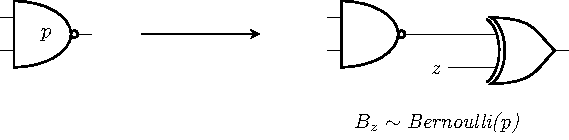
\includegraphics[scale=0.8]{fig/prob-design-eval/prob-distillation.pdf}
    \end{figure}
  \end{block}
  \pause
  \begin{block}{Example: SPBN}
    A standardized PBN with $V_I=\{x_1,x_2,x_3\}$ and $V_O=\{o\}$:
    \begin{figure}
      \centering
      \begin{circuitikz}[scale=0.7, transform shape]
    % Logic gates
    \node[and port] (y1) {$y_1'$};
    \node[xor port,right = of y1, anchor=in 1] (y3) {$y_3$};
    \node[or port,right = of y3, anchor=in 1] (y2) {$y_2$};
    % Wires
    \draw (y1.out) -- (y3.in 1);
    \draw (y3.out) -- (y2.in 1);
    % Labels
    \node[left = 0.1cm of y1.in 1] {$x_1$};
    \node[left = 0.1cm of y1.in 2] {$x_2$};
    \node[left = 0.1cm of y2.in 2] {$x_3$};
    \node[right = 0.1cm of y2.out] {$o$};
    \node[left = 0.1cm of y3.in 2] {$z_1$};
\end{circuitikz}
    \end{figure}
    \begin{itemize}
      \item $p_{z_1}=0.25;p_{y_1'}=p_{y_3}=0$
    \end{itemize}
  \end{block}
\end{frame}
\subsection{Probabilistic Property Evaluation}
\begin{frame}
  \frametitle{Solving PEC and MPEC}
\end{frame}
\subsection{Evaluation}
\subsection{Preliminaries}
\begin{frame}
    \frametitle{Preliminaries}
    \begin{block}{Definition: Exist-Random Quantified SSAT (E-MAJSAT)}
        $\Qf=\exists X,\random{} Y.\pf(X,Y)$
        \pause
        \begin{itemize}
            \item $X$ and $Y$: two disjoint sets of Boolean variables
                  \pause
            \item $\pf(X,Y)$: a CNF formula
                  \pause
        \end{itemize}
    \end{block}
    \begin{block}{Definition: Clause Selection}
        Given a CNF formula $\pf(X,Y)$:
        \pause
        \begin{itemize}
            \item $C=\cx\lor\cy$
                  \pause
            \item An assignment $\as$ over $X$ \textit{selects} $C$ if $\as$ falsifies every literal in $\cx$
                  \pause
            \item Selection variable: $\sv{C}\equiv\lnot\cx$
                  \pause
            \item Selection relation: $\select(X,S)=\bigwedge\limits_{C\in\pf}(\sv{C}\equiv\lnot\cx)$
        \end{itemize}
    \end{block}
\end{frame}

\begin{frame}
    \frametitle{Preliminaries}
    \begin{block}{Example: Clause Selection}
        Consider $\pf(X,Y)$ over $X=\{e_1,e_2,e_3\}$ and $Y=\{r_1,r_2,r_3\}$:
        \begin{itemize}
            \item[] $C_1: (e_1 \lor r_1 \lor r_2)$ $C_2: (e_1 \lor e_2 \lor r_1 \lor r_2 \lor \lnot r_3)$
            \item[] $C_3: (\lnot e_2 \lor \lnot e_3 \lor r_2 \lor \lnot r_3)$ $C_4: (\lnot e_1 \lor e_3 \lor r_3)$
        \end{itemize}
        \pause
        The selection relation $\select(X,S)$ of $\pf(X,Y)$ equals:
        \belowdisplayskip=0pt
        \begin{align*}
            (\sv{1} \equiv \lnot e_1) \land
            (\sv{2} \equiv \lnot e_1 \land \lnot e_2) \land
            (\sv{3} \equiv e_2 \land e_3) \land
            (\sv{4} \equiv e_1 \land \lnot e_3)
        \end{align*}
        \pause
        \begin{itemize}
            \item $\as=\lnot e_1 \lnot e_2 \lnot e_3$: $\pcf{\select}{\as}=s_1s_2\neg s_3 \neg s_4$
        \end{itemize}
    \end{block}
\end{frame}
\subsection{Decision Procedure}
\subsection{Evaluation}
\chapter{Exist-Random Quantified SSAT}
\label{chap:exist-random-ssat}
\chapter{Dependency SSAT}
\label{chap:dependency-ssat}

In this chapter, we lift SSAT to the NEXPTIME-complete complexity class by formulating \textit{dependency SSAT} (DSSAT).
Most content in this chapter is based on our conference paper~\cite{LeeAAAI21DSSAT} published at AAAI '21.

\begin{frame}
    \frametitle{Preliminaries}
    \begin{block}{Definition: Exist-Random Quantified SSAT (E-MAJSAT)}
        $\Qf=\exists X,\random{} Y.\pf(X,Y)$
        \pause
        \begin{itemize}
            \item $X$ and $Y$: two disjoint sets of Boolean variables
                  \pause
            \item $\pf(X,Y)$: a CNF formula
                  \pause
        \end{itemize}
    \end{block}
    \begin{block}{Definition: Clause Selection}
        Given a CNF formula $\pf(X,Y)$:
        \pause
        \begin{itemize}
            \item $C=\cx\lor\cy$
                  \pause
            \item An assignment $\as$ over $X$ \textit{selects} $C$ if $\as$ falsifies every literal in $\cx$
                  \pause
            \item Selection variable: $\sv{C}\equiv\lnot\cx$
                  \pause
            \item Selection relation: $\select(X,S)=\bigwedge\limits_{C\in\pf}(\sv{C}\equiv\lnot\cx)$
        \end{itemize}
    \end{block}
\end{frame}

\begin{frame}
    \frametitle{Preliminaries}
    \begin{block}{Example: Clause Selection}
        Consider $\pf(X,Y)$ over $X=\{e_1,e_2,e_3\}$ and $Y=\{r_1,r_2,r_3\}$:
        \begin{itemize}
            \item[] $C_1: (e_1 \lor r_1 \lor r_2)$ $C_2: (e_1 \lor e_2 \lor r_1 \lor r_2 \lor \lnot r_3)$
            \item[] $C_3: (\lnot e_2 \lor \lnot e_3 \lor r_2 \lor \lnot r_3)$ $C_4: (\lnot e_1 \lor e_3 \lor r_3)$
        \end{itemize}
        \pause
        The selection relation $\select(X,S)$ of $\pf(X,Y)$ equals:
        \belowdisplayskip=0pt
        \begin{align*}
            (\sv{1} \equiv \lnot e_1) \land
            (\sv{2} \equiv \lnot e_1 \land \lnot e_2) \land
            (\sv{3} \equiv e_2 \land e_3) \land
            (\sv{4} \equiv e_1 \land \lnot e_3)
        \end{align*}
        \pause
        \begin{itemize}
            \item $\as=\lnot e_1 \lnot e_2 \lnot e_3$: $\pcf{\select}{\as}=s_1s_2\neg s_3 \neg s_4$
        \end{itemize}
    \end{block}
\end{frame}
\section{Clause-containment learning for E-MAJSAT}
\label{sect:erssat-technique}

Consider an E-MAJSAT formula $\Qf = \exists X,\random{} Y.\pf$.
To obtain the satisfying probability of $\Qf$,
it suffices to enumerate every assignment $\as$ over $X$ and calculate the corresponding conditional satisfying probability $\spb{\pcf{\Qf}{\as}}$.
Clearly, the above brute-force approach is computationally expensive.
Motivated by the idea of clause selection discussed above,
we propose \textit{clause-containment learning} to prune the search space.
The proposed learning technique deduces useful information after each trial of an assignment $\as$ over $X$.
The learnt information is recorded as blocking clauses to avoid wasteful exploration and thus accelerates the search process.
The proposed learning technique is based on the following key observation.

\begin{proposition}
    \label{prop:erssat-contain}
    Given an E-MAJSAT formula $\Qf=\exists X,\random{} Y.\pf(X,Y)$ and two assignments $\as_1,\as_2$ over $X$,
    we have:
    \begin{align*}
        (\pcf{\pf}{\as_2}\models\pcf{\pf}{\as_1})\limply\spb{\pcf{\Qf}{\as_2}}\leq\spb{\pcf{\Qf}{\as_1}}.
    \end{align*}
\end{proposition}

Inspired by~\cref{prop:erssat-contain},
we propose clause-containment learning based on clause selection.
After cofactoring $\pf$ with an arbitrary assignment $\as_1$ over $X$,
a set of clauses $\pcf{\pf}{\as_1}$ is selected.
For any other assignment $\as_2$ selecting all clauses from $\pcf{\pf}{\as_1}$,
i.e., $\pcf{\pf}{\as_1}\subseteq\pcf{\pf}{\as_2}$,
we have $\pcf{\pf}{\as_2} \models \pcf{\pf}{\as_1}$.
Therefore, $\spb{\pcf{\Qf}{\as_2}}\leq\spb{\pcf{\Qf}{\as_1}}$ holds according to~\cref{prop:erssat-contain}.
Since the satisfying probability $\spb{\pcf{\Qf}{\as_2}}$ is not greater than $\spb{\pcf{\Qf}{\as_1}}$,
the assignment $\as_2$ is not worth trying.
For all such assignments,
they should be blocked after $\as_1$ has been explored.

The core concept of the clause-containment learning is to avoid every unexplored assignment $\as_2$ that selects a clause set $\pcf{\pf}{\as_2}$ containing another clause set $\pcf{\pf}{\as_1}$ selected by an explored assignment $\as_1$.
To block the assignment $\as_2$,
we enforce at least one of the clauses in $\pcf{\pf}{\as_1}$ to be deselected.
Recall that the selection variable $\sv{C}$ of clause $C$ valuates to $\bot$ if and only if $C$ is deselected.
Therefore, the disjunction of the negation of the selection variables for the clauses in $\pcf{\pf}{\as_1}$ is deduced as a learnt clause to record this information.
The above idea gives rise to~\cref{alg:erssat} for E-MAJSAT formulas.
(\Cref{code:erssat-subsume-table,code:erssat-minimal-clauses,code:erssat-subsume-clauses,code:erssat-discard-literals} describe the enhancement techniques of the proposed algorithm, which will be discussed later.)

\begin{algorithm}[p]
    \caption{Solving E-MAJSAT formulas}
    \label{alg:erssat}
    \begin{algorithmic}[1]
        \REQUIRE $\Qf=\exists X,\random{} Y.\pf(X,Y)$
        \ENSURE $\spb{\Qf}$
        \STATE $\select(X,S) := \bigwedge\limits_{C\in\pf}(\sv{C}\equiv\lnot\cx)\land\bigwedge\limits_{\text{pure }l: \vl{l}\in X}l$\label{code:erssat-init-select}
        \STATE $prob := 0$
        \STATE $\texttt{s-table} := \texttt{BuildSubsumptionTable}(\pf)$\label{code:erssat-subsume-table}
        \WHILE{($\sat{\select}$)}
        \STATE $\as := \model{\select}$ (discarding the selection variables)
        \IF{($\sat{\pcf{\pf}{\as}}$)}
        \STATE $\as' := \texttt{SelectMinimalClauses}(\pf,\select)$\label{code:erssat-minimal-clauses}
        \STATE $\varphi := \texttt{RemoveSubsumedClauses}(\pcf{\pf}{\as'},\texttt{s-table})$\label{code:erssat-subsume-clauses}
        \STATE $prob := \max\{prob,\texttt{ComputeWeight}(\random{} Y.\varphi)\}$\label{code:erssat-wmc}
        \STATE $C_S := \bigvee\limits_{C\in\varphi}\lnot\sv{C}$
        \STATE $C_L := \texttt{DiscardLiterals}(\pf,C_S,prob)$\label{code:erssat-discard-literals}
        \ELSE
        \STATE $C_L := \texttt{MinimalConflicting}(\pf,\as)$
        \ENDIF
        \STATE $\select := \select \land C_L$
        \ENDWHILE
        \RETURN $prob$
    \end{algorithmic}
\end{algorithm}

The algorithm employs two SAT solvers:
one works on the matrix $\pf(X,Y)$ of the input formula,
and the other works on the selection relation $\select(X,S)$ for clauses in $\pf(X,Y)$.
Using the definition of selection variables,
we initialize the selection relation and assert the literals of pure $X$ variables in~\cref{code:erssat-init-select}.
If a variable $e$ in $X$ is pure in $\pf$,
assigning the literals of $e$ to $\top$ deselects the clauses containing $e$,
and does not affect other clauses.
Because the conditional satisfying probability is greater if less clauses are selected,
we can safely assert pure $X$ variables without missing the optimizing solution.

The selection relation is used to select different assignments $\as$ over $X$.
If $\pcf{\pf}{\as}$ is satisfiable,
a weighted model counter is called to compute the conditional satisfying probability $\spb{\random{} Y.\pcf{\pf}{\as}}$.
The blocking clause $C_L$ derived from the containment-learning technique is then conjoined with $\select$ to prevent clauses in $\pcf{\pf}{\as}$ being simultaneously selected again.

On the other hand, suppose $\pcf{\pf}{\as}$ is unsatisfiable.
We can deduce a conjunction of literals from $\as$ responsible for the conflict by using a SAT solver to analyze the conflict~\cite{Een2003Solver,Een2003Incremental}.
In general, the conjunction of literals may not be minimal,
meaning that some literals can be discarded and the conflict remains unaffected.
The subroutine $\texttt{MinimalConflicting}$ makes the conjunction of literals responsible for the conflict minimal as follows.
For each literal $l$ in the conjunction,
temporarily drop $l$ and check whether $\pf(X,Y)$ is still unsatisfiable.
If it is unsatisfiable, discard $l$; otherwise, keep $l$ in the conjunction.
Repeating the above process for every literal makes the conjunction minimal.
Complementing the minimal conjunction of literals yields a learnt clause,
which is then conjoined with the selection relation to block assignments that make $\pf$ unsatisfiable.

When the selection relation becomes unsatisfiable,
it indicates that the space spanned by variables $X$ has been completely searched.
The algorithm will return the encountered maximum conditional satisfying probability,
which equals the satisfying probability of the input E-MAJSAT formula.

We illustrate the working of algorithm $\mathtt{SolveEMAJSAT}$ in the following example.
\begin{example}\label{ex:erssat-basic}
    Continuing~\cref{ex:erssat-select},
    we show how~\cref{alg:erssat} (without the enhancement techniques) solves the E-MAJSAT instance
    \begin{align*}
        \Qf=\exists e_1,\exists e_2,\exists e_3,\random{0.5} r_1,\random{0.5} r_2,\random{0.5} r_3.\pf.
    \end{align*}

    Let the first explored assignment $\as_1$ be $\lnot e_1 \lnot e_2 \lnot e_3$,
    which selects $C_1$ and $C_2$.
    The algorithm derives $\spb{\random{0.5} r_1,\random{0.5} r_2,\random{0.5} r_3.\pcf{\pf}{\as_1}}=0.75$ by invoking a weighted model counter in~\cref{code:erssat-wmc}.
    The learnt clause $C_L=(\lnot s_1 \lor \lnot s_2)$ is conjoined with $\select$ to prevent $C_1$ and $C_2$ being selected simultaneously again.

    Suppose the second explored assignment $\as_2$ is $\lnot e_1 e_2 \lnot e_3$,
    which selects $C_1$.
    The weighted model counter returns $\spb{\random{0.5} r_1,\random{0.5} r_2,\random{0.5} r_3.\pcf{\pf}{\as_2}}=0.75$,
    and the learnt clause $C_L=(\lnot s_1)$ is conjoined with $\select$ to prevent $C_1$ being selected again.

    Let the third tried assignment $\as_3$ be $e_1 e_2 \lnot e_3$,
    which selects $C_4$.
    The weighted model counter gives $\spb{\random{0.5} r_1,\random{0.5} r_2,\random{0.5} r_3.\pcf{\pf}{\as_3}}=0.5$,
    and the learnt clause $C_L=(\lnot s_4)$ is conjoined with $\select$ to prevent $C_4$ being selected again.

    Let the fourth tried assignment $\as_4$ be $e_1 e_2 e_3$,
    which selects $C_3$.
    The conditional satisfying probability $\spb{\random{0.5} r_1,\random{0.5} r_2,\random{0.5} r_3.\pcf{\pf}{\as_4}}$ equals $0.75$,
    and the learnt clause $C_L=(\lnot s_3)$ is conjoined with $\select$ to prevent $C_3$ being selected again.

    Suppose the fifth tried assignment $\as_5$ is $e_1 \lnot e_2 e_3$,
    which deselects every clause, making $\pcf{\pf}{\as_5}=\top$ and
    $\spb{\random{0.5} r_1,\random{0.5} r_2,\random{0.5} r_3.\pcf{\pf}{\as_5}}=1$.
    Since there is no selected clause,
    the learnt clause $C_L$ is empty,
    and the selection relation becomes unsatisfiable after being conjoined with an empty clause.
    The unsatisfiability of the selection relation reveals that the space spanned by variables $X$ has been exhaustively searched,
    and the algorithm returns the satisfying probability, which equals $1$, of the E-MAJSAT instance.
\end{example}

\subsection{Enhancement techniques}
The efficiency of~\cref{alg:erssat} is greatly affected by the strength of the learnt clauses.
We introduce three enhancement methods,
\textit{minimal clause selection},
\textit{clause subsumption}, and
\textit{partial assignment pruning},
to strengthen the learnt clauses deduced by the proposed learning technique.
In~\cref{alg:erssat},
the enhancement techniques are executed by subroutines
$\texttt{SelectMinimalClauses}$ (in~\cref{code:erssat-minimal-clauses}),
$\texttt{RemoveSubsumedClauses}$ (in~\cref{code:erssat-subsume-clauses}), and
$\texttt{DiscardLiterals}$ (in~\cref{code:erssat-discard-literals}),
to be detailed in the following three parts, respectively.
%Examples~\ref{ex:minimal},~\ref{ex:subsume}, and ~\ref{ex:partial} will be used to explain the three techniques.
%(Please refer to Examples~\ref{ex:minimal},~\ref{ex:subsume},~\ref{ex:partial} in the supplement.)

\subsubsection{Minimal clause selection}
As discussed before,
the selection relation $\select(X,S)$ is in charge of choosing an assignment $\as$ over variables $X$ and thus selects a set of clauses from the matrix $\pf(X,Y)$.
However, the set of selected clauses may not be minimal,
meaning that it is possible for another assignment $\as'$ to select a set of clauses contained in that selected by $\as$, i.e., $\pcf{\pf}{\as'}\subset\pcf{\pf}{\as}$.
Notice that the length of a learnt clause equals the number of selected clauses.
Therefore, selecting fewer clauses gives a stronger learnt clause,
as well as a higher conditional satisfying probability.

Starting from a set of initially selected clauses $\pcf{\pf}{\as}$,
the first enhancement technique \textit{minimal clause selection} decreases the number of selected clauses by making the set of initially selected clauses minimal as follows.
A learnt clause $C_S=\bigvee\limits_{C\in\pcf{\pf}{\as}}\lnot\sv{C}$ is conjoined with the selection relation $\select(X,S)$ to avoid clauses in $\pcf{\pf}{\as}$ being selected simultaneously again.
A SAT solver is invoked to solve $\select\land C_S$ under an assumption $\mu=\bigwedge\limits_{C\notin\pcf{\pf}{\as}}\lnot\sv{C}$.
The assumption $\mu$ prevents originally deselected clauses being selected.
If $\select\land C_S$ under the assumption $\mu$ is satisfied by some assignment $\as'$ over $X$,
the set of clauses selected by $\as'$ must be a proper subset of that selected by $\as$.
On the other hand, if $\select\land C_S$ under the assumption $\mu$ is unsatisfiable,
then the set of selected clauses is minimal.
To make the set of initially selected clauses minimal,
the above operation is repeated until the selection relation becomes unsatisfiable.

The subroutine $\texttt{SelectMinimalClauses}$ for the technique is described in~\cref{alg:erssat-minimal}.
The following example illustrates how this technique improves the solving efficiency.

\begin{algorithm}[p]
    \caption{\texttt{SelectMinimalClauses}}
    \label{alg:erssat-minimal}
    \begin{algorithmic}[1]
        \REQUIRE The matrix $\pf(X,Y)$ and selection relation $\select(X,S)$
        \ENSURE An assignment $\as'$ that selects a minimal set of clauses from $\pf$
        \REPEAT
        \STATE $\as' := \model{\select}$ (discarding the selection variables)
        \STATE $C_S := \bigvee\limits_{C\in\pcf{\pf}{\as'}}\lnot\sv{C}$
        \STATE $\select := \select \land C_S$
        \STATE $\mu := \bigwedge\limits_{C\notin\pcf{\pf}{\as'}}\lnot\sv{C}$
        \UNTIL{($\unsat{\pcf{\select}{\mu}}$)}
        \RETURN $\as'$
    \end{algorithmic}
\end{algorithm}

\begin{example}
    \label{ex:erssat-minimal}
    Continue~\cref{ex:erssat-basic}.
    The first tried assignment $\as_1=\lnot e_1 \lnot e_2 \lnot e_3$ selects $C_1$ and $C_2$.
    The set of selected clauses is made minimal as follows.
    The subroutine $\texttt{SelectMinimalClauses}$ conjoins the selection relation with a learnt clause $(\lnot \sv{1} \lor \lnot \sv{2})$,
    which prevents clauses $C_1$ and $C_2$ being simultaneously selected again.
    The satisfiability of the selection relation $\select\land(\lnot \sv{1} \lor \lnot \sv{2})$ is tested under an assumption $\lnot \sv{3} \lnot \sv{4}$,
    which avoids the originally deselected clause $C_3$ and $C_4$ being selected.
    The formula is satisfied by the assignment $\as_2=\lnot e_1 e_2 \lnot e_3$, which only selects $C_1$.
    By repeating the above operation again,
    the assignment $\as_5=e_1 \lnot e_2 e_3$ is found,
    since it selects no clause.
    The conditional satisfying probability under $\as_5$, which equals $1$,
    is derived without invoking a weighted model counter.
    Compared to~\ref{ex:erssat-basic} where five assignments over $X$ were explored,
    the algorithm with the minimal clause selection technique finds the optimal assignment $\as_5$ with at most two SAT calls,
    thus greatly improves the computation efficiency.
\end{example}

\subsubsection{Clause subsumption}
The second enhancement technique, named \textit{clause subsumption},
decreases the length of a learnt clause via examining the subsumption relation among the selected clauses.
Recall that clause $C_1$ \textit{subsumes} clause $C_2$ if every literal appears in $C_1$ also appears in $C_2$.
Consider a CNF formula $C_1 \land C_2$ with $C_2$ subsumed by $C_1$.
It can be simplified to $C_1$ because $C_2$ is implied by $C_1$ due to the subsumption relation.

The subsumption relation among sub-clauses consisting of variables in $Y$ is constructed as a lookup table by the subroutine $\mathtt{BuildSubsumeTable}$.
The subroutine $\texttt{RemoveSubsumedClauses}$ simplifies the set of selected clauses $\pcf{\pf}{\as}$ by removing subsumed clauses.
A clause $C$ is removed from the set of selected clauses $\pcf{\pf}{\as}$ if $C^Y$ is subsumed by other selected sub-clauses.
We emphasize that, without cofactoring $\pf$ with the assignment $\as$,
the original clauses may not have the subsumption relation.
Cofactoring $\pf$ with the assignment $\as$ over variables in $X$ induces the subsumption relation between sub-clauses consisting of variables in $Y$.

\iffalse
    The procedure $\mathtt{RemoveSubsumedClauses}$ for the technique is outlined in Figure~\ref{fig:subsume}.
    It takes the set of selected clauses and the lookup table of subsumption relation as input, and removes every subsumed clause via subroutine $\mathtt{CheckSubsumption}$.
    \begin{figure}[h]
        \mbox{}\hrulefill \vspace{-.6em}
        \small
        \begin{program}
            \>  {\bf \textit{RemoveSubsumedClauses}}\\
            \> \> \INPUT: The selected clauses $\phi|_{\tau}$ and a lookup table \texttt{s-table}\\ \> \> \> \> \> for subsumption\\
            \> \> \OUTPUT: A simplified set of clauses $\varphi$ without subsumed clasues\\
            \> \> \BEGIN\\
            \> \> 01 \> \> $\varphi$ := $\top$;\\
            \> \> 02 \> \> \FOREACH $C \in \phi|_{\tau}$\\
            \> \> 03 \> \> \> \IF \> $\mathtt{CheckSubsumption}(C,\texttt{s-table})$\\
            \> \> 04 \> \> \> \> \CONTI;\\
            \> \> 05 \> \> \> \ELSE\texttt{//$C^Y$ is not subsumed}\\
            \> \> 06 \> \> \> \> $\varphi$ := $\varphi \wedge C$;\\
            \> \> 07 \> \> \RETURN $\varphi$;\\
            \> \> \END
        \end{program}
        \vspace{-1.2em} \mbox{}\hrulefill \caption{\small Subroutine: Removing subsumed clauses from the set of selected clauses.}
        \label{fig:subsume}
    \end{figure}
\fi

\iffalse
    \begin{example}\label{ex:subsume}
        Continue Example~\ref{ex:basic}.
        Let the first tried assignment be $\tau_1=\neg e_1 \neg e_2 \neg e_3$.
        It selects $C_1$ and $C_2$.
        Because $C_1^Y$ subsumes $C_2^Y$, $C_2$ is removed from $\phi|_{\tau_1}$, yielding $\varphi=C_1$.
        The weighted model counter gives $\Pr[\invR^{0.5}Y.\varphi]=0.75$, and the learnt clause $C_L=(\neg s_1)$ is conjoined with $\psi$ to prevent $C_1$ being selected again.
        Compared to Example~\ref{ex:basic}, with the help of clause subsumption, the learnt clause $(\neg s_1)$ deduced from $\tau_1$ is stronger than its counterpart $(\neg s_1 \vee \neg s_2)$ in Example~\ref{ex:basic}, and therefore avoids a fruitless trail of the assignment $\tau_2=\neg e_1 e_2 \neg e_3$.
    \end{example}
\fi

\subsubsection{Partial assignment pruning}
To illustrate the third enhancement technique \textit{partial assignment pruning},
we first take a closer look at the learnt clause deduced by the proposed clause containment learning.
Given a matrix $\pf(X,Y)$ and an assignment $\as$ over $X$,
a learnt clause consists of the negation of the selection variables of the selected clauses.
For each selected clause $C$,
if the selection variable $\sv{C}$ is substituted by its definition $\sv{C}\equiv\lnot\cx$,
the learnt clause $C_L$ becomes the disjunction of the sub-clauses $\cx$,
i.e., $C_L=\bigvee\limits_{C\in\pcf{\pf}{\as}}\cx$.

For instance, in~\cref{ex:erssat-basic},
the learnt clause deduced from the assignment $\as_1=\lnot e_1 \lnot e_2 \lnot e_3$,
which selects clauses $C_1$ and $C_2$,
is $(\lnot s_1 \lor \lnot s_2)=(e_1 \lor e_2)$,
and the current maximum satisfying probability equals $0.75$.
This learnt clause blocks two assignments, $\as_1$ and $\lnot e_1 \lnot e_2 e_3$.
The assignment $\lnot e_1 \lnot e_2 e_3$ selects clauses $C_1$, $C_2$, and $C_4$,
containing previously selected clauses $C_1$ and $C_2$, and thus is blocked.

A learnt clause is strengthened if some literal in the clause is discarded.
In the above example,
the learnt clause $(e_1 \lor e_2)$ can be strengthened by discarding literal $e_2$.
The resulted learnt clause $(e_1)$ blocks any assignment assigning $e_1$ to $\bot$.
To see why these assignments are blocked,
observe that assigning $e_1$ to $\bot$ selects clause $C_1$.
Although the set $\{C_1\}$ does not contain the previously selected set of clauses $\{C_1,C_2\}$,
the conditional satisfying probability is bounded from above by the probability of the sub-clause $(r_1 \lor r_2)$,
which equals $0.75$.
Since the current maximum satisfying probability equals $0.75$ already,
it is fruitless to explore assignments whose conditional satisfying probabilities are no greater than $0.75$. Therefore, $e_1$ is forced to be $\top$.

On the other hand,
literal $e_1$ cannot be discarded from the learnt clause $(e_1 \lor e_2)$.
If $e_1$ is discarded,
the resulted learnt clause $(e_2)$ blocks any assignment assigning $e_2$ to $\bot$.
However, assigning $e_2$ to $\bot$ selects no clause,
and hence the upper bound of the conditional satisfying probability equals $1$.
Since $1$ is greater than the current maximum satisfying probability $0.75$,
we have to explore assignments assigning $e_2$ to $\bot$.
In fact, there exists an assignment $e_1 \lnot e_2 \lnot e_3$ whose conditional satisfying probability equals $1$,
greater than the current maximum satisfying probability.
As a result, $e_1$ cannot be discarded.

From the above illustration,
we observe that the learnt clause can be strengthened as follows.
First, temporarily discard some literal $l$ in the learnt clause.
Second, invoke a weighted model counter to compute the conditional satisfying probability contributed by the selected clauses.
Third, compare the probability to the current maximum satisfying probability.
If the probability is no greater, literal $l$ is discarded; otherwise, it is kept in the clause.
Fourth, repeat the above steps for other literals.

\iffalse
    The subroutine $\mathtt{DiscardLiterals}$ of the technique to discard literals from a learnt clause is outlined in Figure~\ref{fig:partial}.
    \begin{figure}[h]
        \mbox{}\hrulefill \vspace{-.6em}
        \small
        \begin{program}
            \>  {\bf \textit{DiscardLiterals}}\\
            \> \> \INPUT: The matrix $\phi$, the learnt clause $C_S$,\\
            \> \> \> \> \> and the current max. sat. \texttt{prob}\\
            \> \> \OUTPUT: A strengthened learnt clause $C_L$\\
            \> \> \BEGIN\\
            \> \> 01 \> \> $C_L$ := $\bot$;\\
            \> \> 02 \> \> \FOREACH $s_C \in C_S$\\
            \> \> 03 \> \> \> $C_L$ := $C_L \vee C^X$;\\
            \> \> 04 \> \> \FOREACH $l \in C_L$\\
            \> \> 05 \> \> \> $\nu$ := $\bigwedge_{k \in C_L \setminus \{l\}}\neg k$;\\
            \> \> 06 \> \> \> \IF \> $\mathtt{WeightModelCount}(\invR Y.\phi|_{\nu}) \leq \texttt{prob}$\\
            \> \> 07 \> \> \> \> $C_L$ := $C_L \setminus \{l\}$;\\
            \> \> 08 \> \> \RETURN $C_L$;\\
            \> \> \END
        \end{program}
        \vspace{-1.2em} \mbox{}\hrulefill \caption{\small Subroutine: Discarding literals from a learnt clause.}
        \label{fig:partial}
    \end{figure}

    The subroutine $\mathtt{DiscardLiterals}$ works as follows.
    It substitutes selection variables in the learnt clause $C_S$ by their definitions in lines~\texttt{02-03}.
    Then it iterates through each literal $l \in C_L$, and invokes the weighted model counter to check whether literal $l$ can be discarded in lines~\texttt{04-07}.
    Notice that the current maximum satisfying probability is \emph{not} updated by the value returned from the weighted model counter, because the value only reflects an upper bound for satisfying probabilities under the partial assignment $\nu$.
\fi

\iffalse
    \begin{example}\label{ex:partial}
        Continue Example~\ref{ex:basic}. As discussed above, the learnt clause $(e_1 \vee e_2)$ deduced from the assignment $\tau_1=\neg e_1 \neg e_2 \neg e_3$ is strengthen to $(e_1)$ by the partial assignment pruning technique, and thus prevents a fruitless trail of the assignment $\tau_2=\neg e_1 e_2 \neg e_3$.
    \end{example}
\fi

To summarize, the above three enhancement techniques are designed based on different reasoning strategies:
the minimal clause selection technique strengthens the learnt clause by invoking additional SAT calls to solve the selection relation to select a minimal set of clauses;
the clause subsumption technique builds a lookup table to record the subsumption relation and removes subsumed clauses;
the partial assignment pruning technique utilizes the current maximum conditional satisfying probability,
and invokes extra calls to a weighted model counter to test whether it is feasible to discard some literal in a learnt clause.
Benefiting from the three enhancement techniques,
the efficiency of the proposed algorithm is greatly improved,
as will be shown in our experiments.

We emphasize two more strengths of the proposed algorithm.
First, during the computation,
the proposed algorithm keeps deriving lower bounds for the satisfying probability,
and the bounds gradually converge to the final answer.
Therefore, in contrast to previous DPLL-based methods~\cite{Majercik1998,Majercik2003,Majercik2005},
the proposed algorithm can be easily modified to solve \textit{approximate SSAT} by returning the greatest encountered lower bound upon timeout.
Second, the proposed algorithm is efficient in memory usage,
since it stores the learnt information compactly via selection variables,
and the weighted model counting is invoked on selected clauses,
whose sizes are typically much smaller than that of original matrix.
%In our empirical evaluation, the selected clauses on average account for less than $20\%$ of the entire CNF formula.
%As will be clear from our experimental data, the proposed algorithm improves memory efficiency by more than one order of magnitude compared to previous approaches.

%We emphasize that, the proposed three enhancement techniques are orthogonal to each other. Simultaneously enabling all of them gives the enhanced algorithm in Figure~\ref{fig:enhance}.

\subsection{Implementation details}
We discuss some details about our implementation of the proposed algorithm.
\Cref{alg:erssat} involves satisfiability testing and weighted model counting.
In principle, any SAT solver and exact weighted model counter can be plugged into the procedure.
Therefore, \cref{alg:erssat} may benefit directly from the advancement of SAT solving and model counting.

Specifically in our implementation,
we adopt \texttt{Minisat-2.2}~\cite{Een2003Solver} for SAT solving.
We experimented with \cachet~\cite{Sang2004,Sang2005ModelCounting} for weighted model counting,
but the overall performance was not satisfactory.
Because the clauses selected by different assignments typically share a portion of identical sub-formulas,
the results of these sub-formulas should be cached to avoid repeated computations.
Ideally, this improvement can be achieved by tightly integrating \cachet into our implementation,
instead of treating it as a black box.
However, we resort to \textit{binary decision diagram} (BDD) for our weighted model counting to achieve the \textit{formula caching} effect.

The selected clauses in a formula are first transformed into a two-level circuit by \disjoin-ing literals in each clause and \conjoin-ing the outputs of each \disjoin gate.
A BDD is then constructed based on the resulted circuit.
Weighted model counting of the original formula is done by traversing the BDD~\cite{LeeTC18ProbDesign}.
We use the well-developed BDD package \texttt{CUDD}~\cite{CUDD},
which caches BDD nodes during building BDDs for different formulas.
Thus the formula caching effect,
as well as garbage collection which removes unreferenced nodes,
is automatically achieved by \cudd.

%In our empirical evaluation,
%the formula caching effect improves the runtime by an average of $14\%$ over random CNF formulas,
%and in some cases it improves the efficiency by one order of magnitude.
Our implementation was integrated in the \abc~\cite{ABC}environment,
which provides all the facilities including SAT solving, circuit construction, and BDD computation mentioned above.
\section{Applications of DSSAT}
\label{sect:dssat-application}

In this section, we demonstrate two applications of DSSAT.

\subsection{Analyzing probabilistic/approximate partial design}
After formulating DSSAT and proving its NEXPTIME-completeness,
we show its application to the analysis of probabilistic design and approximate design.
Specifically, we consider the probabilistic version of the \textit{topologically constrained logic synthesis problem}~\cite{Sinha2002,Balabanov2014},
or equivalently the \textit{partial design problem}~\cite{Gitina2013}.

In the \textit{(deterministic) partial design problem},
we are given a specification function $G(X)$ over primary input variables $X$ and
a \textit{partial design} $C_F$ with black boxes to be synthesized.
The Boolean functions induced at the primary outputs of $C_F$ can be described by $F(X,T)$,
where $T$ corresponds to the variables of the black box outputs.
Each black box output $t_i$ is specified with its input variables (i.e., dependency set) $\dep{i}\subseteq X \cup Y$ in $C_F$,
where $Y$ represents the variables for intermediate gates in $C_F$ referred to by the black boxes.
The partial design problem aims at deriving the black box functions $\{h_1(\dep{1}),\ldots,h_{|T|}(\dep{|T|})\}$
such that substituting $t_i$ with $h_i$ in $C_F$ makes the resultant circuit function equal $G(X)$.
The above partial design problem can be encoded as a DQBF problem;
moreover, the partial equivalence checking problem is shown to be NEXPTIME-complete~\cite{Gitina2013}.

Specifically, the DQBF that encodes the partial equivalence checking problem is of the form:
\begin{align}
    \label{eq:dssat-dqbf-partial-design}
    \forall X,\forall Y,\exists T(D).(Y \equiv E(X)) \limply (F(X,T)\equiv G(X)),
\end{align}
where $D$ consists of $(\dep{1},\ldots,\dep{|T|})$,
$E$ corresponds to the defining functions of $Y$ in $C_F$,
and the operator ``$\equiv$'' denotes element-wise equivalence between its two operands.

The above partial design problem can be extended to its probabilistic variant,
which is illustrated by the circuit shown in \textbf{TODO}.
The \textit{probabilistic partial design problem} is the same as the deterministic partial design problem except that
$C_F$ is a distilled probabilistic design~\cite{LeeTC18ProbDesign} with black boxes,
whose functions at the primary outputs can be described by $F(X,Z,T)$,
where $Z$ represents the variables for the auxiliary inputs that trigger errors in $C_F$
(including the errors of the black boxes) and
$T$ corresponds to the variables of the black box outputs.
Each black box output $t_i$ is specified with its input variables (i.e., dependency set)
$\dep{i} \subseteq X \cup Y$ in $C_F$.
When $t_i$ is substituted with $h_i$ in $C_F$,
the function of the resultant circuit is required to be sufficiently close to the specification with respect to some expected probability.

\begin{theorem}
    The probabilistic partial design problem is NEXPTIME-complete.
\end{theorem}
\begin{proof}
    To show that the probabilistic partial design problem is in the NEXPTIME complexity class,
    we note that the black box functions can be guessed and validated in time exponential to the number of black box inputs.

    To show completeness in the NEXPTIME complexity class,
    we reduce the known NEXPTIME-complete DSSAT problem to the probabilistic partial design problem,
    similar to the construction used in the previous work~\cite{Gitina2013}.
    Given a DSSAT instance,
    it can be reduced to a probabilistic partial design instance in polynomial time as follows.
    Without loss of generality,
    consider the DSSAT formula~\cref{eq:dssat}.
    We create a probabilistic partial design instance by letting the specification $G$ be a tautology and
    letting $C_F$ be a probabilistic design with black boxes,
    which involves primary inputs $x_1,\ldots,x_n$ and black box outputs $y_1,\ldots,y_m$ to compute the matrix $\pf$.
    The driving inputs of the black box output $y_j$ is specified by the dependency set $\dep{y_j}$ in~\cref{eq:dssat},
    and the probability for primary input $x_i$ to evaluate to $\top$ is set to $p_i$.
    The original DSSAT formula is satisfiable with respect to a target satisfying probability $\theta$ if and only if
    there exist implementations of the black boxes such that the resultant circuit composed with the black box implementations behaves like a tautology with respect to the required expectation $\theta$.
\end{proof}

On the other hand,
the probabilistic partial design problem can be encoded with the following XDSSAT formula:
\begin{align}
    \label{eq:dssat-partial-design}
    \random{} X,\random{} Z,\forall Y,\exists T(D).(Y \equiv E(X)) \limply (F(X,Z,T)\equiv G(X)),
\end{align}
where the primary input variables are randomly quantified with probability $p_{x_i}$ of $x_i \in X$ to reflect their weights,
and the error-triggering auxiliary input variables $Z$ are randomly quantified according to the pre-specified error rates of the erroneous gates in $C_F$.
Notice that the above formula takes advantage of the extension with universal quantifiers as discussed previously.

In approximate design,
a circuit implementation may deviate from its specification by a certain extent.
The amount of deviation can be characterized in a way similar to the error probability calculation in probabilistic design.
For approximate partial design,
the equivalence checking problem can be expressed by the XDSSAT formula:
\begin{align}
    \label{eq:dssat-approximate-design}
    \random{} X,\forall Y,\exists T(D).(Y \equiv E(X)) \limply (F(X,T)\equiv G(X)),
\end{align}
which differs from~\cref{eq:dssat-partial-design} only in requiring no auxiliary inputs.
The probabilities of the randomly quantified primary input variables are determined by the approximation criteria in measuring the deviation.
For example, when all the input assignments are of equal weight,
the probabilities of the primary inputs are all set to 0.5.

We note that as the engineering change order (ECO) problem~\cite{JiangDATE20ECOSurvey} heavily relies on partial design equivalence checking,
the above DSSAT formulations provide fundamental bases for ECOs of probabilistic and approximate designs.
\chapter{Conclusion and Future Work}
\label{chap:conclusion-future-work}

In this dissertation,
the research needs highlighted in~\cref{chap:introduction} have been addressed.
Specifically,
the applicability of SSAT to the analysis of VLSI systems was examined.
We formulated a framework for the property evaluation of probabilistic design,
and encoded the average-case and the worst-case analyses
as random-exist and exist-random quantified SSAT formulas, respectively.

Motivated by the emerging VLSI applications,
we further designed novel algorithms for random-exist and exist-random quantified SSAT formulas.
The proposed algorithms aim at leveraging the success from SAT/QBF-solving and model-counting communities,
so as to advance the state-of-the-art of SSAT solving beyond the conventional DPLL-based search.
For random-exist quantified SSAT formulas,
we used minterm generalization and weighted model counting as subroutines,
and employed SAT solvers and weighted model counters as plug-in engines.
For exist-random quantified SSAT formulas,
we devised the clause-containment learning,
which was inspired by the clause-selection technique of QBF.
Under the framework of clause-containment learning,
three clause-strengthening heuristics were proposed to improve the computational efficiency.
Moreover, unlike previous exact SSAT methods,
the proposed algorithms can solve approximate SSAT by deriving upper and lower bounds of satisfying probability.
Experiment results showed the benefits of our solvers over a wide range of benchmarking instances.
Our implementations and the benchmark suite of SSAT instances are open-source
for other researchers to base their work on top of our results.

To generalize SSAT beyond the PSPACE-complete complexity class for more complex problems,
we extended DQBF to its stochastic variant DSSAT and proved its NEXPTIME-completeness.
Compared to the PSPACE-complete SSAT,
DSSAT is more powerful to succinctly model NEXPTIME-complete decision problems with uncertainty.
We demonstrated the DSSAT formulation of the analysis to probabilistic/approximate partial design,
and gave a polynomial-time reduction from the NEXPTIME-complete Dec-POMDP to DSSAT.

For future work,
we plan to incorporate Monte-Carlo simulation into our framework of probabilistic property evaluation,
and develop solvers for arbitrary quantified SSAT and DSSAT formulas.
We note that the clause-containment learning has been generalized to solve general SSAT~\cite{Chen2021},
and the recent developments of DQBF~\cite{Tentrup2019} might provide a promising framework for DSSAT solving.

\iffalse
    We have proposed a formal framework to probabilistic property
    evaluation, under the worst-case and average-case scenarios.
    Connections between probabilistic property evaluation and existing
    solving techniques have been established. A novel BDD-based SSAT solver is proposed. A comparative experimental study has been performed to assess the capabilities
    of different methods. Among the considered solutions, the proposed BDD-based SSAT solver, which makes use of circuit structures to construct BDD, currently tends to be the most robust in our experiments. Nevertheless, there are cases solvable only by approximate weighted model counting, but not by other methods. As the BDD-based method has its memory explosion problem, SSAT and model
    counting approaches based on CNF formula might be more viable than the BDD one if their efficiency would be improved in the future. Our results may benefit the synthesis of probabilistic design, perhaps not only for silicon but also for genetic circuits, which are intrinsically stochastic. For future investigation, Monte-Carlo simulation may be incorporated to our proposed formal methods.

    In this paper, we focused on solving random-exist quantified SSAT formulas.
    In contrast to the previous DPLL-based algorithms, we proposed a novel algorithm using SAT solver and weighted model counter as underlying engines to improve computational efficiency.
    Leveraging the great success of modern SAT solving techniques, the proposed algorithm outperforms the state-of-the-art method in the experiment on random $k$-CNF and strategic companies formulas.
    Moreover, unlike previous exact SSAT methods, the proposed algorithm can be easily modified to solve approximate SSAT by deriving upper and lower bounds of satisfying probability.
    We demonstrated the applicability of our SSAT solver to VLSI circuit analysis.
    While the state-of-the-art solver fails to compute the exact satisfying probability, the proposed method succeeded in finding bounds of the formulas.
    In several cases, the derived bounds are very close to, or even match the exact satisfying probability.
    This approximation flexibility of our method can be helpful when SSAT is applied to real-world applications.
    %This work might shed light on the application of solving approximate SSAT to real-world problems.
    For future work, we intend to extend the proposed algorithm to arbitrary quantified SSAT formulas.

    We developed a new approach to solving E-MAJSAT formulas. In contrast to prior methods based on DPLL search or knowledge compilation, we proposed the clause containment learning technique, inspired by clause selection recently developed in QBF evaluation, and design a novel algorithm to solve E-MAJSAT efficiently. Under the framework of clause containment learning, three enhancement techniques were proposed to improve the computational efficiency.
    Experiment results show the benefit of our method.
    %that our method achieves significant performance gains and memory savings over prior SSAT methods, and also provides useful lower bound information for cases where no information can be given by prior methods.
    For future work, we intend to solve SSAT with general prefix structure.

    In this paper, we extended DQBF to its stochastic variant DSSAT and proved its NEXPTIME-completeness.
    Compared to the PSPACE-complete SSAT, DSSAT is more powerful to succinctly model NEXPTIME-complete decision problems with uncertainty.
    The new formalism can be useful in applications such as artificial intelligence and system design.
    Specifically, we demonstrated the DSSAT formulation of the analysis to probabilistic/approximate partial design, and gave a polynomial-time reduction from the NEXPTIME-complete Dec-POMDP to DSSAT.
    We envisage the potential broad applications of DSSAT and plan solver development for future work.
    %\textcolor{blue}{
    We note that recent developments of \textit{clausal abstraction} for QBF~\cite{JanotaM15,RabeT15} and DQBF~\cite{Tentrup19} might provide a promising framework for DSSAT solving.
    Clausal abstraction has been lifted to SSAT~\cite{ChenHJ21}, and we are investigating its feasibility for DSSAT.
    %}
\fi

%---------------------------------------------------

% Add list of figures (handled by package tocbibind)
\listoffigures
% Add list of tables (handled by package tocbibind)
\listoftables
% Add list of algorithms (manually register this list to ToC)
\cleardoublepage
\phantomsection
\addcontentsline{toc}{chapter}{List of Algorithms}
\listofalgorithms
% Add bibliography (handled by package tocbibind)
\bibliographystyle{acm}
\bibliography{nzlee,prob}

\end{document}